\def\paperversiondraft{draft}
\def\paperversionnormal{normal}

% If the paper version is set to 'normal' mode keep it,
% otherwise set it to 'draft' mode.
\ifx\paperversion\paperversionnormal
\else
  \def\paperversion{draft}
\fi

\documentclass[acmsmall,screen,review]{acmart}

% \def\acmversionanonymous{anonymous}
% \def\acmversionjournal{journal}
% \def\acmversionnone{none}

% \makeatletter
% \if@ACM@anonymous
%   \def\acmversion{anonymous}
% \else
%   \def\acmversion{journal}
% \fi
% \makeatother

% \usepackage{colortbl}

% % 'draftonly' environment
% \usepackage{environ}
% \ifx\paperversion\paperversiondraft
% \newenvironment{draftonly}{}{}
% \else
% \NewEnviron{draftonly}{}
% \fi

% Most PL conferences are edited by conference-publishing.com. Follow their
% advice to add the following packages.
%
% The first enables the use of UTF-8 as character encoding, which is the
% standard nowadays. The second ensures the use of font encodings that support
% accented characters etc. (Why should I use this?). The mictotype package
% enables certain features 'to­wards ty­po­graph­i­cal per­fec­tion
% \usepackage[utf8]{inputenc}
% \usepackage[T1]{fontenc}
% \usepackage{microtype}

% \usepackage{xargs}
% \usepackage{lipsum}
% \usepackage{xparse}
% \usepackage{xifthen, xstring}
% \usepackage{xspace}
\usepackage{marginnote}
% \usepackage{etoolbox}
\usepackage{acronym}
\usepackage{cleveref}
\usepackage{subcaption}
\usepackage{listings}
\usepackage{amsmath}
% \usepackage{thmtools} % required for autoref to lemmas
\usepackage{algorithm}
\usepackage{algorithmicx}
\usepackage{tabularx}

\usepackage{mathtools}
\usepackage{siunitx}
\usepackage{makecell}
% \usepackage[svgnames]{xcolor}
% \usepackage{minted}

\input{tex/setup.tex}
\input{tex/acm.tex}

% \usemintedstyle{colorful}

% Newer versions of minted require the 'customlexer' argument for custom lexers
% whereas older versions require the '-x' to be passed via the command line.
\makeatletter
\ifcsdef{MintedExecutable}
{
  % minted v3
  \newminted[mlir]{tools/lexers/MLIRLexer.py:MLIRLexerOnlyOps}{mathescape}
  \newminted[xdsl]{tools/lexers/MLIRLexer.py:MLIRLexer}{mathescape, style=murphy}
  \newminted[lean4]{tools/lexers/Lean4Lexer.py:Lean4Lexer}{mathescape}
}
{
  \ifcsdef{minted@optlistcl@quote}
  {
    \newminted[mlir]{tools/lexers/MLIRLexer.py:MLIRLexerOnlyOps}{customlexer, mathescape}
    \newminted[xdsl]{tools/lexers/MLIRLexer.py:MLIRLexer}{customlexer, mathescape, style=murphy}
    \newminted[lean4]{tools/lexers/Lean4Lexer.py:Lean4Lexer}{customlexer, mathescape}
  }
  {
    \newminted[mlir]{tools/lexers/MLIRLexer.py:MLIRLexerOnlyOps -x}{mathescape}
    \newminted[xdsl]{tools/lexers/MLIRLexer.py:MLIRLexer -x}{mathescape, style=murphy}
    \newminted[lean4]{tools/lexers/Lean4Lexer.py:Lean4Lexer -x}{mathescape}
  }
}
\makeatother

% We use the following color scheme
%
% This scheme is both print-friendly and colorblind safe for
% up to four colors (including the red tones makes it not
% colorblind safe any more)
%
% https://colorbrewer2.org/#type=qualitative&scheme=Paired&n=4

\definecolor{pairedNegOneLightGray}{HTML}{cacaca}
\definecolor{pairedNegTwoDarkGray}{HTML}{827b7b}
\definecolor{pairedOneLightBlue}{HTML}{a6cee3}
\definecolor{pairedTwoDarkBlue}{HTML}{1f78b4}
\definecolor{pairedThreeLightGreen}{HTML}{b2df8a}
\definecolor{pairedFourDarkGreen}{HTML}{33a02c}
\definecolor{pairedFiveLightRed}{HTML}{fb9a99}
\definecolor{pairedSixDarkRed}{HTML}{e31a1c}

\createtodoauthor{grosser}{pairedOneLightBlue}
\createtodoauthor{healy}{pairedTwoDarkBlue}
\createtodoauthor{luisa}{pairedThreeLightGreen}
\createtodoauthor{authorFour}{pairedFourDarkGreen}
\createtodoauthor{arjun}{pairedFiveLightRed}
\createtodoauthor{christos}{pairedSixDarkRed}
\createtodoauthor{kuhn}{pairedNegTwoDarkGray}

\acrodef{cfg}[CFG]{Control-Flow Graph}
\acrodef{ssa}[SSA]{Static Single Assignment}
\acrodef{ila}[ILA]{Instruction-Level Abstraction}
\acrodef{isa}[ISA]{Instruction Set Architecture}
\acrodef{chc}[CHC]{Constrained Horn Clause}
\acrodef{eda}[EDA]{Electronic Design Automation}
\acrodef{ir}[IR]{Intermediate Representation}
\acrodef{fol}[FOL]{First Order Logic}
\acrodef{fsm}[FSM]{Finite State Machine}
\acrodef{smt}[SMT]{Satisfiability Modulo Theory}
\acrodef{cgra}[CGRA]{Course-Grained Reconfigurable Array}
\acrodef{rtl}[RTL]{Register-Transfer Level}
\acrodef{jit}[JIT]{Just-In-Time}
\acrodef{hls}[HLS]{High-Level Synthesis}
\acrodef{ltl}[LTL]{Linear Temporal Logic}
\acrodef{bmc}[BMC]{Bounded Model Checking}
\acrodef{dsl}[DSL]{Domain-Specific Language}
\acrodef{hdl}[HDL]{Hardware Description Language}

\graphicspath{{./images/}}

% Define macros that are used in this paper

% We require all macros to end with a delimiter (by default {}) to enusure
% that LaTeX adds whitespace correctly.
\makeatletter
\newcommand\requiredelimiter[2][########]{%
  \ifdefined#2%
    \def\@temp{\def#2#1}%
    \expandafter\@temp\expandafter{#2}%
  \else
    \@latex@error{\noexpand#2undefined}\@ehc
  \fi
}
\@onlypreamble\requiredelimiter
\makeatother

\newcommand\newdelimitedcommand[2]{
\expandafter\newcommand\csname #1\endcsname{#2}
\expandafter\requiredelimiter
\csname #1 \endcsname
}

\newdelimitedcommand{toolname}{EDAMAME}

\usepackage{booktabs}
% \newcommand{\ra}[1]{\renewcommand{\arraystretch}{#1}}

% \usepackage[verbose]{newunicodechar}
% \newunicodechar{₁}{\ensuremath{_1}}
% \newunicodechar{₂}{\ensuremath{_2}}
% \newunicodechar{∀}{\ensuremath{\forall}}
% \newunicodechar{α}{\ensuremath{\alpha}}
% \newunicodechar{β}{\ensuremath{\beta}}

% % \circled command to print a colored circle.
% % \circled{1} pretty-prints "(1)"
% % This is useful to refer to labels that are embedded within figures.
% \DeclareRobustCommand{\circled}[2][]{%
%     \ifthenelse{\isempty{#1}}%
%         {\circledbase{pairedOneLightBlue}{#2}}%
%         {\autoref{#1}: \hyperref[#1]{\circledbase{pairedOneLightBlue}{#2}}}%
% }

% % listings don't write "Listing" in autoref without this.
% \providecommand*{\listingautorefname}{Listing}
% \renewcommand{\sectionautorefname}{Section}
% \renewcommand{\subsectionautorefname}{Section}
% \renewcommand{\subsubsectionautorefname}{Section}

\begin{document}

\title[abstraction]{\toolname{}: Hardware Model Checking in the Abstraction Age}
%% As discussed, this title is fun but not very explicit about the topic (and we don't do any explicit state-space evaluation)
%% \title{CIRCT-MC: A state-space Odyssey}

%% Author information
%% Contents and number of authors suppressed with 'anonymous'.
%% Each author should be introduced by \author, followed by
%% \authornote (optional), \orcid (optional), \affiliation, and
%% \email.
%% An author may have multiple affiliations and/or emails; repeat the
%% appropriate command.
%% Many elements are not rendered, but should be provided for metadata
%% extraction tools.
% \author{First1 Last1}
% \authornote{with author1 note}          %% \authornote is optional;
% %% can be repeated if necessary
% \orcid{nnnn-nnnn-nnnn-nnnn}             %% \orcid is optional
% \affiliation{
%   \position{Position1}
%   \department{Department1}              %% \department is recommended
%   \institution{Institution1}            %% \institution is required
%   \streetaddress{Street1 Address1}
%   \city{City1}
%   \state{State1}
%   \postcode{Post-Code1}
%   \country{Country1}
% }
% \email{first1.last1@inst1.edu}          %% \email is recommended

% \author{First2 Last2}
% \authornote{with author2 note}          %% \authornote is optional;
% %% can be repeated if necessary
% \orcid{nnnn-nnnn-nnnn-nnnn}             %% \orcid is optional
% \affiliation{
%   \position{Position2a}
%   \department{Department2a}             %% \department is recommended
%   \institution{Institution2a}           %% \institution is required
%   \streetaddress{Street2a Address2a}
%   \city{City2a}
%   \state{State2a}
%   \postcode{Post-Code2a}
%   \country{Country2a}
% }
% \email{first2.last2@inst2a.com}         %% \email is recommended
% \affiliation{
%   \position{Position2b}
%   \department{Department2b}             %% \department is recommended
%   \institution{Institution2b}           %% \institution is required
%   \streetaddress{Street3b Address2b}
%   \city{City2b}
%   \state{State2b}
%   \postcode{Post-Code2b}
%   \country{Country2b}
% }
% \email{first2.last2@inst2b.org}         %% \email is recommended

\begin{abstract}

  % An abstract should consist of six main sentences:
  %  1. Introduction. In one sentence, what’s the topic?
  Modern \ac{eda} tools empower designers to create complex hardware with greater productivity than ever before. \arjun{The first sentence feels a little strange to me, like are they really "creating" hardware, or something}
  As hardware complexity continues to increase, though, verifying the hardware we design is becoming progressively more challenging, and we are beginning to see the limits of testbench-based verification.
    %  2. State the problem you tackle.
  Formally verifying hardware provides strong guarantees of correctness, but
  comes at significant computational cost that scales poorly with design size.
  %  3. Summarize (in one sentence) why nobody else has adequately answered the research question yet.
  Inductive model checking algorithms have made great strides in reducing this
  bottleneck, but are ultimately limited in how much information they can
  extract from the \ac{rtl} designs they traditionally receive.
  %  4. Explain, in one sentence, how you tackled the research question.
  Hence, we argue that focusing on general-purpose model-checking algorithms is no longer the best fit for today's hardware design processes.
  Hardware compilers increasingly provide high-level abstractions to improve designer productivity, but the structural information encoded in these abstractions is usually discarded in the verification process.
  Instead, we propose building verification models from the high-level representations of the designs, allowing tools to make informed choices about the algorithms they use.
  %  5. In one sentence, how did you go about doing the research that follows from your big idea.
  By providing verification tooling with both a general-purpose RTL model checking algorithm and domain-specific algorithms, model checkers can verify faster without loss of generality.
  %  6. As a single sentence, what’s the key impact of your research?
  In this paper, we explore how a dedicated verification algorithm can be used to create a model checker that can verify any RTL design, but can also exploit explicit high-level finite state machine descriptions to provide faster verification times.
  We demonstrate this approach with \toolname{}, a model checker built on the CIRCT framework, and show that it achieves a 35.8\% reduction (geomean) in model-checking time on real-world finite state machines over state-of-the-art RTL model checkers.

  % (http://www.easterbrook.ca/steve/2010/01/how-to-write-a-scientific-abstract-in-six-easy-steps/)
\end{abstract}

% Only add ACM notes and keywords in camera ready version
% Drop citations and footnotes in draft and blind mode.
% \ifx\acmversion\acmversionanonymous
%   \settopmatter{printacmref=false} % Removes citation information below abstract
%   \renewcommand\footnotetextcopyrightpermission[1]{} % removes footnote with conference information in first column
% \fi

% \ifx\acmversion\acmversionjournal
%   %% 2012 ACM Computing Classification System (CSS) concepts
%   %% Generate at 'http://dl.acm.org/ccs/ccs.cfm'.
%   \begin{CCSXML}
%     <ccs2012>
%     <concept>
%     <concept_id>10011007.10011006.10011008</concept_id>
%     <concept_desc>Software and its engineering~General programming languages</concept_desc>
%     <concept_significance>500</concept_significance>
%     </concept>
%     <concept>
%     <concept_id>10003456.10003457.10003521.10003525</concept_id>
%     <concept_desc>Social and professional topics~History of programming languages</concept_desc>
%     <concept_significance>300</concept_significance>
%     </concept>
%     </ccs2012>
%   \end{CCSXML}

%   \ccsdesc[500]{Software and its engineering~General programming languages}
%   \ccsdesc[300]{Social and professional topics~History of programming languages}
%   %% End of generated code

%   %% Keywords
%   %% comma separated list
%   \keywords{keyword1, keyword2, keyword3}
% \fi

%% \maketitle
%% Note: \maketitle command must come after title commands, author
%% commands, abstract environment, Computing Classification System
%% environment and commands, and keywords command.
\maketitle

\section{Introduction}
%https://docs.google.com/drawings/d/10er9hoqEd7plWkHKglRiU2ZM8l2--GmrLL4rrr-YIkw/edit?usp=sharing
\begin{figure}
  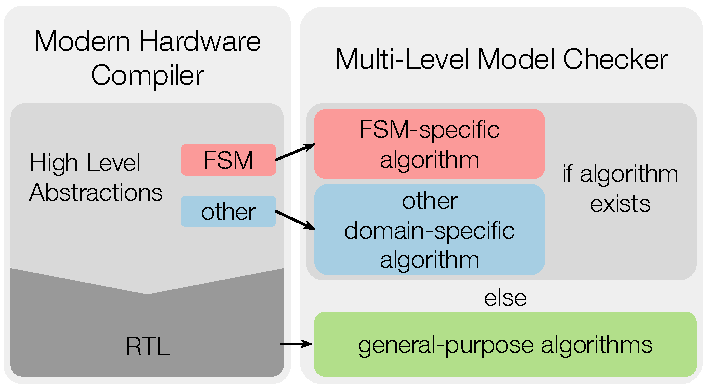
\includegraphics[width=0.8\columnwidth]{core-idea.pdf}
  \caption{We propose providing a tool with domain-specific algorithms to verify designs with high-level abstractions, falling back to general-purpose model checking algorithms when no applicable domain-specific algorithm is known.} \label{fig:intro-verif}
\end{figure}

Around half of the development effort involved in hardware design is spent on verification~\cite{wilson2018verifstudy, wilson2020verifstudy, wilson2022verifstudy}, taking up valuable engineer time that would otherwise be spent on designing and implementing novel hardware.
Much of this verification is done with simulation and testbenches.
This style of verification is vital, but has clear limitations.
Fundamentally, a simulation can only explore the cases that occur to the testbench developer, so bugs can easily go unnoticed if that engineer does not think of a particular corner case.

Formal verification tackles this by considering every possible execution a piece of hardware could undergo.
This allows us to gain completeness, but at a cost --- the entire state space of a design must be considered, which grows exponentially with the size of the design.
Various approaches have been taken to mitigate the impact of this state-space explosion~\cite{Clarke2001, clarke2012explosion, nejati2021explosion}, but ultimately all hit a limit in the amount of information an \ac{rtl} design can encode.
We argue that this bottleneck need not exist --- in fact, we are closer to overcoming it than we realize thanks to the abstractions in hardware compilers that, in part, allowed designer productivity and hardware complexity to rise in the first place.

Modern hardware compilers offer designers higher levels of abstraction in response to the increasing complexity of modern hardware.
Hardware compilers~\cite{calyx, mlir_circt}, \ac{hls} tools~\cite{xilinx_hls, heterohalide, halide_hls, zhang2024optimizing} and domain-specific hardware description languages~\cite{hlhdl, dahlia, chen2024allo} allow designers to iterate over a more abstract view of the hardware without concerning themselves with low-level implementation details.
Each of these approaches introduces a high-level abstraction in the hardware description that provides valuable structural information that could guide the verification process, yet this information is typically discarded at the verification stage.
We believe that these abstractions should be used in tandem with domain-specific verification algorithms to select the best verification strategy for a given design.
A standard RTL \ac{bmc} algorithm~\cite{bmc_found_1} can provide completeness, but is unnecessarily slow and wasteful on designs with a known higher-level structure.
Contrastingly, domain-specific algorithms can verify certain designs much faster~\cite{bogor, cascading_verification}, but are only applicable to a subset of designs --- clearly, these two can be combined to each complement the weaknesses of the other.

We propose a model checker adapted to the multi-level nature of modern hardware design flows.
\kuhn{This claims that the general principle of using multi-level knowledge can speed up model-checking, but we really only focus on  FSMs as the key abstraction. Are there other abstractions used in hardware that can be used as evidence to support the claim that using multi-level representations is a general technique and not specific to only FSMs? I'm not saying we need to remove this claim, but I think it would be nice to add 2-3 more exampels of this technique to substsantiate this claim.}
We describe the architecture of a bounded model checker built upon explicit intermediate representations for model checking, and discuss how this can be complemented with an alternative model checking technique for one of the most widely-used constructs in digital hardware: \acp{fsm}.
We demonstrate that a model checker can be built which combines the strengths of both of these approaches by implementing our idea in the CIRCT framework~\cite{CIRCT}, a hardware compiler ecosystem that provides various high-level abstractions, including an explicit \ac{fsm} representation.

\vspace{.5em}
\noindent
Our contributions are:
\begin{itemize}
  \item A modular architecture for an RTL model checker built on explicit IRs for model checking (\autoref{sec:bmc})
  \item A model checking technique for designs described in a high-level \ac{fsm} representation using \acp{chc} (\autoref{sec:smt-gen})
  \item Techniques for performing bounded translation validation of the \ac{chc} models generated from \acp{fsm} by proving their equivalence with the lowered RTL model of the same FSM (\autoref{sec:tv}).
  \item An RTL-to-FSM extraction algorithm verified correct on the real-world OpenTitan FSMs and a dataset/benchmark of real-world FSMs. (\Cref{sec:fsm-extraction})
  \item A demonstration that model checking techniques can be combined to achieve both completeness and performance with \toolname{}, a model checker built in the CIRCT framework (\autoref{sec:eval})
  \item An evaluation of \toolname{} on RTL designs and various synthetic and real-world \acp{fsm}, achieving a 35.8\% reduction in model-checking time on real-world \acp{fsm} over rIC3, the winner of the 2024 Hardware Model Checking Competition (\autoref{sec:eval})
  \kuhn{We have EDAMAME-FSM and EDAMAME-RTL, but is there any sense in which they work together/synergise? For example, if there is a design that has an RTL input to an FSM, can we use EDAMAME-FSM to check the FSM part and EDAMAME RTL to check the RTL part. This is not just a hypothetical: this situation actually happens in \href{https://github.com/lowRISC/opentitan/blob/d8b5efd1427152b8387d6e03d9db413167e58475/hw/top_englishbreakfast/ip_autogen/pwrmgr/rtl/pwrmgr_fsm.sv}{pwrmgr\_fsm.sv} on the input \texttt{slow\_lc\_done}}
\end{itemize}

% reset acronyms for re-expansion before backgroun
\acresetall

\section{Background}
As this work bridges topics in compilers, EDA tooling and formal verification,
we provide background on each.

\subsection{Abstraction in Hardware Compilation}
Following the rise of high-level languages in the software world, we are seeing a trend towards raising the level of abstraction for hardware designers.
\ac{hls} tools~\cite{cong2022hls} generate hardware from a high-level imperative description (often a software language subset) and domain-specific \acp{hdl} equip hardware compilers with architectural information.
These approaches rely on good compilers, thus hardware compilers are evolving to model the high-level concepts seen in these new front-ends.
Some \ac{hls} compilers provide \acp{ir} that natively model dataflow and scheduling, and \acp{ir} like Calyx~\cite{calyx} and HIR~\cite{majumder2021hir} encode abstract views of hardware to enable new optimizations.

Historically, new hardware abstractions and IRs have been represented in disjoint, incompatible frameworks.
LLHD~\cite{schuiki2020llhd} proposed instead using SSA form~\cite{cytron1991efficiently}, an IR form where each variable can be assigned to only once, as a common representation for building hardware IRs.
We operate upon a multi-level variant of SSA, where operations and types are split into \textit{dialects} to distinguish between the abstraction they represent --- specifically, we use the implementation of this concept found in the CIRCT framework~\cite{CIRCT, mlir_circt} (which is based on MLIR~\cite{mlir}).
CIRCT's IR represents RTL in its \textit{core dialects}: \texttt{comb} for combinational logic, \texttt{seq} for stateful sequential logic and \texttt{hw} for hardware organization and structure.
An example of such IR can be seen below:
% minipage to avoid text being split across paragraphs
% \begin{minipage}[t][26pt]{\columnwidth}
%   \vspace*{0.5mm}
\begin{xdsl}
  %0 = comb.add %1, %2 : i32
\end{xdsl}
% \end{minipage}
% \vspace*{0mm}
% \christos{instead of this fake syntax notation/placeholder, I'd use the \texttt{comb} example from below}
This example performs the the \texttt{add} operation from the \texttt{comb} dialect on two values (\texttt{\%1} and \texttt{\%2} --- values in SSA are traditionally prefixed with a ``\texttt{\%}'') and assigns the result to \texttt{\%0}.
The type of the result is specified after the ``\texttt{:}'' sign.
The assignment can be omitted where an operation does not return a result or its result is not needed.
Some operations specify custom syntax, e.g., by using a keyword to identify certain operands.
For instance, the \texttt{seq.compreg} operation, which defines a register, specifies reset values explicitly: 
\begin{xdsl}
  %0 = seq.compreg %1 reset %reset_signal,
                            %reset_value : i32
\end{xdsl}
Some operations also have \textit{regions} associated with them, each of which intuitively describes a sequence of operations that can be executed by the parent region.
The \texttt{hw.module} operation is an example of this --- it describes a hardware module, and has a region describing the module's contents.
We build upon CIRCT as it uses these concepts to provide various high-level abstractions for digital hardware, making it an ideal platform to demonstrate our approach

\begin{figure}
\begin{subfigure}[T]{0.5\columnwidth}
  \begin{mlir}
  fsm.machine @fsm10() -> (i4) attributes {initialState = "A"} {
    %cnt = fsm.variable "cnt" {initValue = 0 : i4} : i4
    %c0 = hw.constant 0 : i4
    %c1 = hw.constant 1 : i4
    %c5 = hw.constant 5 : i4
    fsm.state @A output {
      fsm.output %cnt : i4
    } transitions { 
      fsm.transition @B
    }
    fsm.state @B( ) output {
      fsm.output %cnt : i4
    } ( )transitions {
      fsm.transition @A guard {
        %isFive = comb.icmp eq %cnt, %c5 : i1
        fsm.return %isFive
      } action {
        fsm.update %cnt, %c0 : i4
      }
      fsm.transition @B guard {
        %isntFive = comb.icmp ne %cnt, %c5 : i1
        fsm.return %isntFive
      } action {
        %newCnt = comb.add %cnt, %c1 : i4
        fsm.update %cnt, %newCnt : i4
      }
    }
  }
  \end{mlir}
\end{subfigure}
\hfill
\begin{subfigure}[T]{0.3\columnwidth}
  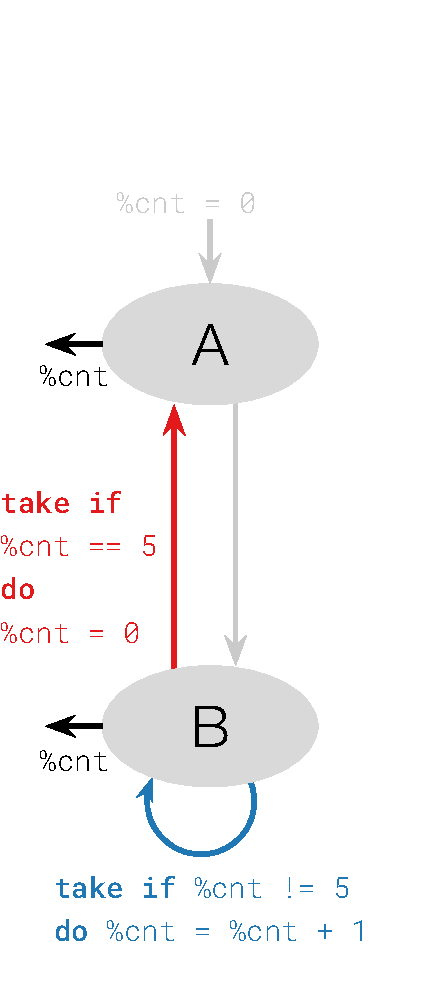
\includegraphics[width=\columnwidth]{fsm-dialect.pdf}
\end{subfigure}
\caption{The operations within CIRCT's \texttt{fsm} dialect describe the structure of a \ac{fsm}. 
We highlight the operations that explicitly capture its behavior.}
\label{fig:fsm-struc}
\end{figure}

  
\subsubsection{FSM Representations}

\acp{fsm} are widely used in digital hardware~\cite{pedroni2013fsms}, and are the near-ubiquitous model for control logic.
Hardware design tooling often infers \acp{fsm}~\cite{giomi1995fsmextraction, shi2010fsmextraction, liu1998fsm} to optimize their transition systems and implementations~\cite{barkalov2021fsmdecomp, barkalov2024fsmreduct}.
For instance, Yosys~\cite{yosys}, a popular open-source synthesis tool, has a dedicated pass for the extraction and optimization of \acp{fsm} found in ingested designs, 
and many other proprietary tools provide similar features~\cite{vivadouserguide, iseguide}.
However, the extraction of FSMs from RTL designs is non-trivial, since implementation details and styles can vary so widely between designs.
As a result, FSM extraction tends to be best effort, and reliant upon FSMs being described in a format specific to the synthesis tool.

Instead, we base our work on CIRCT's \texttt{fsm} dialect, which describes \acp{fsm}' structures by explicitly defining an \ac{fsm}'s states, transitions and outputs (\autoref{fig:fsm-struc}).
An \ac{fsm} contains a set of variables existing within its scope, e.g., \texttt{\%cnt} in \autoref{fig:fsm-struc}. 
Each \texttt{state} operation comprises two regions, describing the output yielded in the state and the transitions starting in that state, respectively. 
Each \texttt{transition} operation itself contains two potentially empty regions, describing the \texttt{guard}, i.e., the condition determining whether the 
transition is taken, and the \texttt{action}, i.e., the set of updates the transition causes on the FSM's variables. 
For example, in \autoref{fig:fsm-struc}, the transition from \texttt{B} to \texttt{A} is only taken when \texttt{\%cnt==5} and, when taken, causes the reset of \texttt{\%cnt} (\texttt{\%cnt=0}).
Instead, the transition from \texttt{B} to \texttt{B} is taken when \texttt{\%cnt!=5} and causes the \texttt{\%cnt} to be incremented by one (\texttt{\%newCnt=comb.add \%cnt,\%c1}).
At the time of writing, this dialect is used as a high-level \ac{ir} for several CIRCT \ac{hls} flows, and is also produced by PyCDE, a CIRCT frontend embedded in Python.

Overall, the \texttt{fsm} dialect provides a high-level description of \acp{fsm}, explicitly representing their core components and high-level structure. 
% \christos{this is a direct reference to the figure, not as advised by our group's style guide. I'd also maybe consider moving this sentence higher up in the paragraph}
% \christos{no strong takeaway point here either}

\subsection{Verification Tooling}
Hardware can be formally verified in several ways -- we describe the techniques relevant to \toolname{} below.

\arjun{You are writign a lot about many different tools, reads a bit like related work more than background to me personally, is all the data about all the diff solvers needed here?}

\subsubsection{SAT and SMT Solvers}
Given a Boolean formula, SAT solvers~\cite{sat_review} determine whether or not there is an assignment of variables under which the formula evaluates to true.
\ac{smt} solvers~\cite{barrett2021satisfiability} extend this problem with several first-order theories
such as quantifiers, arrays and fixed-width bitvectors.
\grosser{cite SAT and SMT solver}
Various SAT and SMT solvers are available with focus on specific theories~\cite{kowalewski2009boolector, niemetz2020bitwuzla}. 
In this work we use Z3~\cite{z3}, which focuses on efficiency in software verification problems and is the only SMT solver provided as an optional dependency of the CIRCT project.\christos{this is the relevant bit here, maybe spend some time to explain the choice and relevance and move other stuff to related work?}

\subsubsection{Model Checking}
Model checking refers to verifying properties of finite state systems, by interpreting the system in a mathematical model, and then checking that properties hold over this model.
These properties take the form of either safety properties (which indicate that some
formula over the model will \textit{always} hold in any reachable state) or liveness
properties (which indicate that something must always \textit{eventually}
happen at some point in the trace).

Bounded model checking~\cite{bmc_found_1} is a commonly used technique for hardware verification.
It uses SAT~\cite{model_checking_foundation0} or \ac{smt} solvers~\cite{smt_instead_of_sat} to confirm that given properties are not violated\grosser{These citations should come earlier}
within an execution of a given length by formulating the system as a set of
logical formulae and proving that there is no state the system can be in that
violates them. This technique provides excellent generality, but often suffers
from state-space explosion~\cite{Clarke2001, clarke2012explosion} --- the space of potential states a design can have increases exponentially as the length of the modelled execution and the size of the design increase.

Inductive model checking techniques are often used to combat this explosion.
They generate an unbounded inductive proof that an invalid state cannot be reached. IC3 (also known as property-directed reachability)~\cite{ic3_original, ic3} is a popular SAT-based inductive model checking
technique used by most of the model checking tools we discuss.

It is common for hardware to be exported in standardized formats and fed to separate model-checking tools.
The existing model checkers we discuss ingest either B\textsc{tor}2~\cite{btor2} or AIGER~\cite{aiger2}.
These formats describe a netlist composed of combinational logic operations and state elements.
CIRCT is equipped with an export pass to B\textsc{tor}2~\cite{amelia_thesis}, which we use to benchmark \toolname{} against other tools (\autoref{sec:eval}).
\christos{similar to previous subsection; I think this can be shortened and made more relevant to our tool}

\begin{figure*}
  \begin{subfigure}[t]{0.48\textwidth}
  \begin{xdsl}
  hw.module @counter(in %clk: !seq.clock,
      in %reset: i1, out count: i32) {
    %c0 = hw.constant 0 : i32
    %c1  = hw.constant 1 : i32
    %reg  = seq.compreg %sum, %clk
                reset %reset, %c0 : i32
    %sum  = comb.add %reg, %c1 : i32
    verif.assert <safety property> : i1
    hw.output %reg : i32
  }
  \end{xdsl}
  \caption{\toolname{}'s RTL engine accepts modules in core CIRCT dialects such as this counter, which outputs \texttt{\%reg}, a register output which increases by one on each clock cycle. Note that \texttt{hw.module} operations contain \emph{graph regions}, allowing the use of \texttt{\%sum}
   in the \texttt{seq.compreg} operation before its definition.}
  \label{lst:counter}
  \end{subfigure}
  \hfill
  \begin{subfigure}[t]{0.48\textwidth}
  \begin{xdsl}
  hw.module @counter(in %clk: !seq.clock,
      in %reset: i1, in %reg_state : i32,
      out count: i32, out reg_next: i32)
      attributes {num_regs = 1} {
    %c1 = hw.constant 1 : i32
    %sum = comb.add %reg_state, %c1 : i32
    verif.assert <safety property> : i1
    hw.output %reg_state, %sum : i32, i32
     
    }
  \end{xdsl}
  \caption{Registers are removed and replaced with module ports. The final input, \texttt{reg\_state}, represents the current state of the register, which is provided to the module. The final output, \texttt{reg\_next}, represents the state the register will assume in the next clock cycle, and is produced by the module.}
  \label{lst:counter-ext-regs}
  \end{subfigure}
  \noindent\begin{subfigure}[t]{0.48\textwidth}
  \begin{xdsl}
  
    %0 = verif.bmc bound 20 num_regs 1 init {
      %false = hw.constant false
      %4     = seq.to_clock %false
      verif.yield %4 : !seq.clock
    } loop {
    ^bb0(%arg0: !seq.clock):
      %4    = seq.from_clock %arg0
      %true = hw.constant true
      %5    = comb.xor %4, %true : i1
      %6    = seq.to_clock %5
      verif.yield %6 : !seq.clock
    } circuit {
    ^bb0(%arg0: !seq.clock, %arg1: i1, %arg2: i32):
      %c1 = hw.constant 1 : i32
      %4      = comb.add %arg2, %c1 : i32
      verif.assert <safety property> : i1
      verif.yield %arg2, %4 : i32, i32
    }
  \end{xdsl}
  \caption{The \texttt{verif.bmc} operation describes a bounded model checking problem. Note that CIRCT does not provide a negation operation, so we negate the clock by XORing with the constant \texttt{true}.}
    \label{lst:counter-bmc-op}
  \end{subfigure}
  \hfill
  \noindent\begin{subfigure}[t]{0.48\textwidth}
  \begin{xdsl}
  
  func.func @bmc_circuit(
        %arg0: !smt.bv<1>,
        %arg1: !smt.bv<1>,
        %arg2: !smt.bv<32>)
            -> (!smt.bv<32>, !smt.bv<32>) {
    %c1 = smt.bv.constant #smt.bv<1> : !smt.bv<32>
    %0 = smt.bv.add %arg2, %c1 : !smt.bv<32>
    %negated_property = smt.not <safety property>
    smt.assert %negated_property
    return %arg2, %0 : !smt.bv<32>, !smt.bv<32>
  }
  
  \end{xdsl}
  \caption{Modules are represented by functions that operate on bitvectors from the \texttt{smt} dialect, and safety properties are negated.}
  \label{lst:counter-smt}
  \end{subfigure}
  \caption{\toolname{}'s RTL pipeline lowers through several levels of abstraction.}
  \label{fig:bmc-pipeline}
  \grosser{Is there any insight/conclusion/claim we want to evidence. Does this relate to some of our key ideas?}
  \end{figure*}
  

\subsubsection{Constrained Horn Clauses}
Finite-state systems are often described as \acp{chc}, which are a fragment of \ac{fol}~\cite{gurfinkel2022program}.
Intuitively, these clauses form an implication stating that if a set of predicates holds true over some arguments, and an additional clause (or constraint) holds over the arguments of these predicates, another predicate must be true over some set of arguments.
% \christos{form an implication stating == imply?}
Formally, these clauses take the form:
\begin{equation}
  \forall V\cdot ( \phi\land p_1(X_1)\land ...\land p_n(X_n)\implies h(X)  )
\end{equation}


where all free variables in the sentence are in \arjun[$V$]{Are they in $V$ or do they take values in $V$? I presume that $V$ is a set of values, not variables.}, $\{p_i\}_{i=1}^n$ and $h$ are uninterpreted predicate symbols, $\{X_i\}_{i=1}^n$ and $X$ are first-order terms over values in $V$ and $\phi$ is some constraint over the variables in $V$.

Equivalently, we can write
a \ac{chc} as:
\begin{equation}
  \neg\phi \lor\neg p_1(X_1)\lor ...\lor\neg p_n(X_n)\lor h(X)
\end{equation}
where all free variables are implicitly universally quantified.
A set of \acp{chc} $\Phi$ is satisfiable if there exists a model $\mathcal{M}$
satisfying $\Phi$, i.e., $\exists\mathcal{M}.\mathcal{M}\models\Phi$.

In this work we use SPACER~\cite{spacer1,spacer2}, Z3's dedicated CHC solver engine, which internally uses a version of IC3.

\section{The \toolname{} RTL Engine}
\label{sec:bmc}
The foundation of our Multi-Level Model Checking approach is an RTL model
checking engine built upon a set of domain-specific IRs, which implements model checking
as a sequence of compiler lowerings that incrementally lower the initial RTL code to
executable code. As a result,
we obtain a modular framework, where changing the algorithm used to
perform model checking is as simple as changing a compiler lowering.

The series of incremental lowerings that make up our RTL model checker
(\autoref{fig:bmc-pipeline}) convert a CIRCT RTL design into a
program that solves a BMC problem.
First, we abstract away the notion of state from an RTL design by eliminating state elements.
Next, we build an explicit representation of the BMC problem that describes the circuit and the behavior of its clocks, without specifying any particular algorithm.
We subsequently lower this problem into a concrete algorithmic implementation
--- this lowering determines the algorithm to be executed.
Finally, we lower this algorithmic representation to an LLVM program that executes the BMC algorithm.

While our prototype implements a simple BMC algorithm, our explicit representation of BMC problems as an IR allows fine-grained, modular algorithmic control not previously available in a unified framework.

\newpage
% \autoref{fig:bmc-pipeline} demonstrates the RTL pipeline, which consists of a series of incremental lowerings through abstraction levels.
% We use a novel, explicit representation of bounded model checking problems that allows fine-grained control over clock behavior in multi-clock designs.
% This representation is then lowered to the SMT dialect.
% We import an existing SMT dialect to CIRCT~\cite{todo}, and use this to build lowerings that directly encode the semantics of CIRCT operations by representing them as SMT formulae.
% \grosser{This claim is heavily predicated. You make this sound like you are first to use an API of CIRCT. You built the first
% model checker in CIRCT which uses a novel design. Did you check with Martin if the SMT dialect in CIRCT has been published, if not then
% the entire SMT dialect is a contribution of this paper. Using an SMT-IR for the implementation of a model-checker,
% independently of CIRCT is then the novely.}
% RTL model checking is not a key contribution of this work, so we implement only a lowering to a simple bounded model checking algorithm.
% \grosser{What is the conclusion here? First, use the 'scientific excuse', it is
% well-known, so we only implemented a standard algorithm which can later serve as
% a foundation for further optimization. Do not downplay your contributions.}

\subsection{\toolname{}'s RTL Pipeline}
\toolname{} starts with a CIRCT RTL design (\autoref{lst:counter}).
This IR describes a simple counter module with a clock input, a reset input, and an output that counts up by one on each clock cycle.
The \texttt{hw.constant} operations define bitvector constants of value 0 and 1 and width 32.
The \texttt{seq.compreg} operation defines a register of width 32 that resets to 0, and the \texttt{comb.add} operation increments the value in this register by 1.
We note that \texttt{seq.compreg} operations are annotated with an additional initial value for simulation/model checking, but we omit this for brevity.
The \texttt{verif.assert} operation defines a safety property over the module's contents that must hold across all checked cycles, and the \texttt{hw.output} operation defines the module's outputs.


\subsubsection{Register Externalization}
The first stage in the RTL pipeline is a preprocessing stage to make representing register states simpler.
SMT solvers have no notion of stateful formulae, so \toolname{} tracks the symbolic states of the registers in the design it is given and provides these to Z3 in a separate SMT problem on each cycle.
To ease this process, \toolname{}'s first transformation \textit{externalizes} all registers within the body of the module --- the output of this transformation when applied to \autoref{lst:counter} is shown in \autoref{lst:counter-ext-regs}.
Intuitively, this can be seen as dragging every register in the design out of the module, without disconnecting its input and output.
The input and output must now flow in and out of the module, so we add ports for these values, then destroy the register and promise to emulate its presence ourselves.
We are left with a module containing no registers, but with an output port describing the register's next state and an input port describing its current state.
\toolname{} then emulates the registers that we externalized from the design.
After externalization, modules are then annotated with a \texttt{num\_regs} attribute indicating how many registers have been externalized --- \toolname{} uses this to determine which ports to treat as registers.

\subsubsection{BMC Operation Generation}
Next, \toolname{} encodes the module explicitly as a bounded model checking problem.
This is represented in the \texttt{verif} dialect as a \texttt{verif.bmc} operation, which describes the circuit to be tested, the number of cycles to check, and the behaviour of the clocks.
We see an example of such an operation in \autoref{lst:counter-bmc-op} (which is generated from the design seen in \autoref{lst:counter}).
The operation first specifies the number of timesteps to check (20 in this case) and the number of registers in the design (1 in this case).
The \texttt{init} region describes how the clock should be initialized --- in this case it is simply set to false.
The \texttt{loop} region describes how the clock should be toggled on each cycle --- in this case, it is simply negated on each cycle with an XOR operation.
The \texttt{init} and \texttt{loop} regions are provided to allow users to describe the clock interleavings when multiple clocks are provided to the module.
When only one clock is found in the module, this clock will be toggled on and off, but to support multiple clocks additional arguments and return values can also be added to indicate, e.g., which clock should be toggled next.
When only one clock is present in the design, we provide a mode that skips cycles where the clock has a falling edge, which most RTL model checkers do.

\subsubsection{\texttt{SMT} Dialect Generation}

Once the bounded model checking problem has been encoded as a \texttt{verif.bmc} operation, it can be lowered to an algorithmic implementation in terms of SMT formulae in the bitvector theory.
We build on the recently introduced idea of modelling IR semantics as an SMT compiler
IR~\cite{mathieu_talk}, using an explicit SMT IR to represent the semantics of CIRCT operations.

We create a function in terms of SMT bitvectors (\autoref{lst:counter-smt}), and surround this with MLIR code describing the model checking algorithm - in the case of our simple BMC algorithm, this executes the \texttt{init} region, then executes the circuit function (along with the contents of the loop region) repeatedly until the bound is reached.
If the solver returns \texttt{sat} at any point, there is a reachable state that violates the safety property, and the property does not hold.
As previously mentioned, this lowering determines the model checking algorithm executed, and an alternative algorithm can be introduced by modifying this lowering.

\subsubsection{LLVM Generation}
Finally, the program must be lowered to LLVM IR for execution.
All operations are converted to MLIR's \texttt{llvm} dialect for export, and \texttt{smt} dialect operations are replaced with calls to the corresponding Z3 API functions.
The remaining LLVM program can be executed directly by \toolname{} using MLIR's just-in-time compilation infrastructure, or can be emitted as LLVM IR directly for cross compilation for another target.

\section{Efficient FSM Model Checking with CHCs}
\label{sec:smt-gen}
We convert \acp{fsm} in CIRCT's \texttt{fsm} dialect into a set of \acp{chc}, allowing us to make use of an efficient domain-specific solver engine.
To do this, we encode the semantics of these operations into SMT formulae in \ac{chc} form.
Conceptually, we translate an \ac{fsm} transition $s_h \rightarrow s_k$ into an implication, with the antecendent describing the transition's starting state $s_h$ and the consequent describing the arriving state $s_k$. We create an uninterpreted boolean function to represent each state:
\begin{equation}
  F_{s_i}: I, O, V, t \rightarrow Bool
\end{equation}
where $I$ contains the FSM's inputs' values, $O$ contains the FSM's outputs' values, $V$ contains the variables' values, and $t$ is an 
integer time value incremented every time a transition is taken.
This discrete time value is particularly valuable for translation validation against RTL models, which we discuss in \autoref{sec:tv}.
The function $F$ returns true if the FSM can be in the state $s_i$ with the given inputs, outputs and variables at the given time. 
Notably, in this model, the state functions indicate the \textit{reachability} of a given state, rather than describing a specific execution.

Transitions can be made conditional using \textit{guards}, regions which return true if the transition is to be taken.
We encode this conditionality by including the guard in the antecedent of guarded transitions $s_h \xrightarrow{\gamma} s_k$:
\begin{align}
  \begin{split}
    &\forall i\in I,\;\forall i'\in I',\;\forall o\in O,\;\forall v\in V \\
    F_{s_h}(i, o, v&, t) \land \gamma(s_h, s_k, v, i) \implies F_{s_k}(i', o', v', t + 1) 
  \end{split}
  \label{eq:transition}
\end{align}
where: 
\begin{itemize}
\item $\gamma(s_h, s_k, v, i)$ is a boolean function representing the condition described in the \texttt{guard} of transition $s_h \xrightarrow{\gamma} s_k$
\item $i'$ represents the next set of inputs to the FSM, 
\item $v'$ contains an updated set of values of the FSM's variables, according to the action function described in the transition $s_h \xrightarrow{\gamma} s_k$  
\item $o'$ contains an updated set of output values, according to the output region specified in state $s_k$ 
\item time $t$ is incremented when the transition is taken
\end{itemize}

Given the values of $i\in I$ and $v\in V$, \Cref{eq:transition} specifies that if state $s_h$ is \textit{reachable} and $\gamma(s_h, s_k, v, i)$ returns true, 
then state $s_k$ is also reachable at the next time-step $t+1$, with a new set of input, output and variable values.

% In \Cref{eq:transition}, the antecedent of the implication (known as the \textit{tail} of the \ac{chc}) requires that the state $s_h$ is reachable with the given inputs, variables and outputs, and that the guard function $\gamma$ is satisfied.
% The precedent of the implication (or the \textit{head} of the \ac{chc}) specifies that if the antecedent is met, the state $s_k$ is reachable at time $t+1$ with the new values for the variables and outputs calculated by $\alpha$ and $\omega$.
Notably, we quantify over all possible inputs on both sides of the implication --- it is this that causes the predicates to represent reachability, rather than a specific execution.
Since the execution is a function of the inputs, we simply need to activate the implication for any possible input to ensure that the predicate is set to true for all reachable states.

Finally, we specify the initial state's reachability:
\begin{equation}
  \forall i\in I,\; t = 0 \implies F_{s_0}(i, v_{0}, o_0, t)
  \label{eq:safety-prop}
\end{equation}
with $v_{0}$ describing the variables' initial values and $o_0$ representing 
the outputs' initial values (calculated from the output region of the initial state).

% \luisa{i dont think the following lines are necessary, since whe specified the reachability above, already}
% Readers may notice that this model only determines a \textbf{necessary} condition for the reachability of a state --- it specifies the conditions under which state's reachability predicate must be true, but not that it can be reached \textit{only} in those cases.
% This means we require safety properties to be specified in a certain form, as discussed below, but allows strict adherence to the \ac{chc} structure, allowing \toolname{} to use the SPACER engine to solve the model very efficiently.

\subsection{Encoding Safety Properties}

A safety property checks that \textit{nothing bad} ever happens in a system --- that is to say, an unsafe state can never be reached.
To disprove a safety property it is sufficient to find a path traversing the \ac{fsm} in which the property does not hold, while to prove it we need to check that the property holds on any possible path through the system.
We encode such properties as \textit{reachability problems} on a certain state $s$ as:

% examples to explain the formula below: 
%  linear fsm: safety prop that holds "c = x at state S"

% (1) forall c, t : (Fs (c, t) && (c != x)) => false (THIS is the one we concretely use)
%     returns SAT --- this means false isn't reachable, which means state S with c != x (bad state) isn't reachable
% (2) forall c, t : (Fs (c, t) && (c == x)) => false
%     returns UNSAT, which means that false could be reached via state S with c == x, so a safe state is reachable

%  linear fsm: safety prop that does not hold "c = y at state x" (with y != x)
% (3) forall c, t : (Fs (c, t) && (c == y)) => false 
%     returns SAT --- false is unreachable because state S with c == y is unreachable
% (4) UNSAT forall c, t : (Fs (c, t) && (c != y)) => false
%     returns UNSAT --- false is reachable because S with c != y is reachable

%  according to the nomenclature below, we have: 

%  safe(c, t) = (c == x)
%  unsafe(c, t) = (c != x)

%  we can rewrite 
%  (1) = forall c, t : (Fs(c, t) && unsafe(c, t)) => false -> S
%  (2) = forall c, t : (Fs(c, t) && safe(c, t)) => false -> U

%  note that with the current (24 feb. 2025) state of the repository, we formulate the properties as (1)
\begin{align}
\begin{split}
  % \begin{split}
    & \forall v\in V, \forall o\in O, \forall i\in I, \forall t\\
    F_s&(i,o,v,t) \land \text{Unsafe}(v, i, o) \implies \bot %\\
  %  & = \neg (F_s(I,V,t) \land \text{Unsafe}(V, I))\lor \bot \\
  %  & = \neg (F_s(I,V,t) \land \text{Unsafe}(V, I)) \\
  %  & = \neg F_s(I,V,t) \lor \neg\text{Unsafe}(V, I) \\
  %  & = \neg F_s(I,V,t) \lor \text{Safe}(V, I) \\
  % \end{split}
\end{split}
\end{align}
The precedent of this implication describes the circumstances in which the property is violated --- if a state $s$ is reachable and the property $\text{Unsafe}(v, i, o)$ holds over the values taken by variables, inputs and outputs in this state, the implication is activated.
The subsequent of this implication is false --- this means that if an unsafe state can be reached, the subsequent (which is false) must be true.
This is trivially unsatisiable, and thus the solver is forced to return \texttt{unsat}.
On the contrary, if the solver returns \texttt{sat}, we can conclude that this implication was never activated, and thus an unsafe state cannot be reached and the safety property holds.
We solve these problems using SPACER~\cite{spacer1,spacer2}, Z3's CHC solver engine.

\section{Verifying the Translation}
\label{sec:tv}

The \ac{chc} encoding of FSMs \toolname{} generates can be verified quickly, but introduces an additional lowering in which trust is vital --- fast model checking is entirely useless if we are not confident the hardware generated from the high-level abstraction will reflect the semantics of the high-level model.
The lowerings used to generate RTL from FSMs are complex, containing hundreds of lines of arbitrary C++ code referencing thousands more lines of MLIR infrastructure, so directly verifying these lowerings is incredibly difficult.
Instead, we complement \toolname{}'s FSM model with a \textit{bounded translation validation} approach using \toolname{}'s \ac{rtl} engine.
By specifying the equivalence of the RTL models and FSM models as a safety property, we can use existing bounded model checking infrastructure to ensure the \ac{chc} models have the expected semantics.
To express this, we assert that the output of the FSM model and the RTL model must always be equivalent on any given cycle - we track the current cycle with a counter circuit.
Throughout this section, we omit conversions between bitvectors and integers for legibility, but Z3 provides functions for these conversions.
For each CHC state predicate, we emit an assertion; for an FSM with no inputs, one output and one variable, such an assertion would be of the form:
\begin{align}
\begin{split}
F(&\texttt{fsm\_v}, \texttt{fsm\_o}, t) \land t = \texttt{timer\_output} \implies \\
&\texttt{fsm\_v} = \texttt{rtl\_v} \land \texttt{fsm\_o} = \texttt{rtl\_o}
\end{split}    
\end{align}
For FSMs with inputs, equivalence over the inputs must also be asserted to ensure that both models are exploring the same trace.
For each input $i$, a function:
\begin{equation}
  I_i : Int \rightarrow Int
\end{equation}    
is instantiated, returning the input's value at a given timestep.
The equivalence of the RTL model's inputs and the input specified by this function is asserted:
\begin{equation}
  I_i(\texttt{timer\_output}) = \texttt{rtl\_input\_0} 
\end{equation}    
and an additional guard clause is inserted on each transition to ensure transitions follow the correct trace.
The SMT problem produced by this procedure combines bitvector and integer theories, making it slow to solve~\cite{xu2021mixedsmt} and unfit for use every time the lowering is used.
Instead, we believe this would be best used in fuzzing, for verifying a large corpus of randomly generated FSMs to increase overall confidence in the correctness of the lowerings.

\section{Real-World FSM Extraction and Benchmark}
\label{sec:fsm-extraction}

We detail a tool and algorithm for extracting FSM structure from an RTL netlist.
This algorithm is inspired by the \texttt{fsm\_extract} pipeline from Yosys (see \href{https://yosyshq.readthedocs.io/projects/yosys/en/0.44/cmd/fsm_extract.html}{fsm\_extract})


\subsection{FSM Extraction Algorithm}
To understand the inputs and the outputs of FSM extraction, see \Cref{fig:fsm-extraction}.
The inputs and outputs are drawn diagrammatically in \Cref{fig:fsm-transformation}

The algorithm works as follows
\begin{enumerate}
  \item Use BFS to explore only reachable states from the initial state
  \item Inline the body of the module, and use canonicalization rules to propagate constants
\end{enumerate}

Backwards constant propagation is added by adding the new rewrite rule
\[if(c,a,b) = n  \xRightarrow[]{isconst(if(c,a,b))}if(c, a = n, b = n)\]

This rewrite rule is only a simplification under the condition $isconst(if(c,a,b))$, which is defined by

\begin{align}
isconst &: Expr \to \mathbb{B}\\
isconst(n) &= true \\
isconst(if(c, a, b)) &= isconst(a) \land isconst (b) \\
isconst(\_) = false
\end{align}

The set of states explored is pruned by using symbolic evaluation of the next state function.
\begin{align}
se &: Expr \to 2^{\mathbb{N}} \\
se(constant(c)) &= \left\{c\right\} \\
se(mux(c,a,b)) &= se(a) \cup se(b) \\
se(\_ : i_{n}) &= \left\{0, 1, 2, 3, \ldots, 2^{n}-2, 2^{n}-1\right\}
\end{align}
The extraction algorithm is described in \Cref{fig:fsm_extraction_workflow}.
The algorithm is explained in pseudo-code in \Cref{alg:fsm_extraction}

% \begin{algorithm}[H]
% \caption{Simplified FSM Extraction from a Hardware Module}
% \label{alg:fsm_extraction}
% \begin{algorithmic}[1]
% \Function{ExtractFSM}{$M : hw.module$}
%   \State initialRegVal : $i_s$ := getInitialRegVal(M)
%   \State nextState : $i_i \to i_s \to i_s$ := getNextStateLogic(M)
%   \State output : $i_s \to i_o$ := getOutputLogic(M)
%   \State workList : List(Int) := [initalRegVal]
%   \State visitedStates : Set(Int) := \{\}
%   \State fsm : FSM := new FSM()
%   \While{workList $\neq$ []}
%   \State cs : $i_s$ := workList.pop()
%   \State $visitedState \gets visitedStates \cup \{cs\}$
%    \State S : State := fsm.addState(cs, output(cs))
%    \State pns : Set($i_s$) := se(nextState(\_, cs))
%    \For{$ns : i_S \in pns$}
%      \State S.addTransition(ns, $i \mapsto nextState(i, cs) = ns$)
%      \If{$ns \notin visitedStates$}
%        \State workList.pushBack(ns)
%      \EndIf
%    \EndFor
% \EndWhile
%   \State \Return fsm
% \EndFunction
% \end{algorithmic}
% \end{algorithm}


\subsection{Performance of FSM Extraction}
The performance scales with $O(n^2)$ with respect to the number of transitions in the FSM.
For a graph of performance, see \Cref{fig:fsm-performance}.

\subsection{Extracting Real-World FSMs}

We extract and verify real-world FSMs. We tested the pass on the FSMs in the OpenTitan Project\footnote{\href{https://github.com/lowRISC/opentitan?tab=readme-ov-file}{github.com/lowRISC/opentitan}}.
See \Cref{tab:fsm_conversion}.
The correctness of the FSMs was verified using \texttt{circt-bmc}.
The verification process is described in \Cref{fig:fsm_extraction_workflow}.

% End of code


\begin{figure*}[ht]
    \begin{subfigure}[t]{0.49\textwidth}

  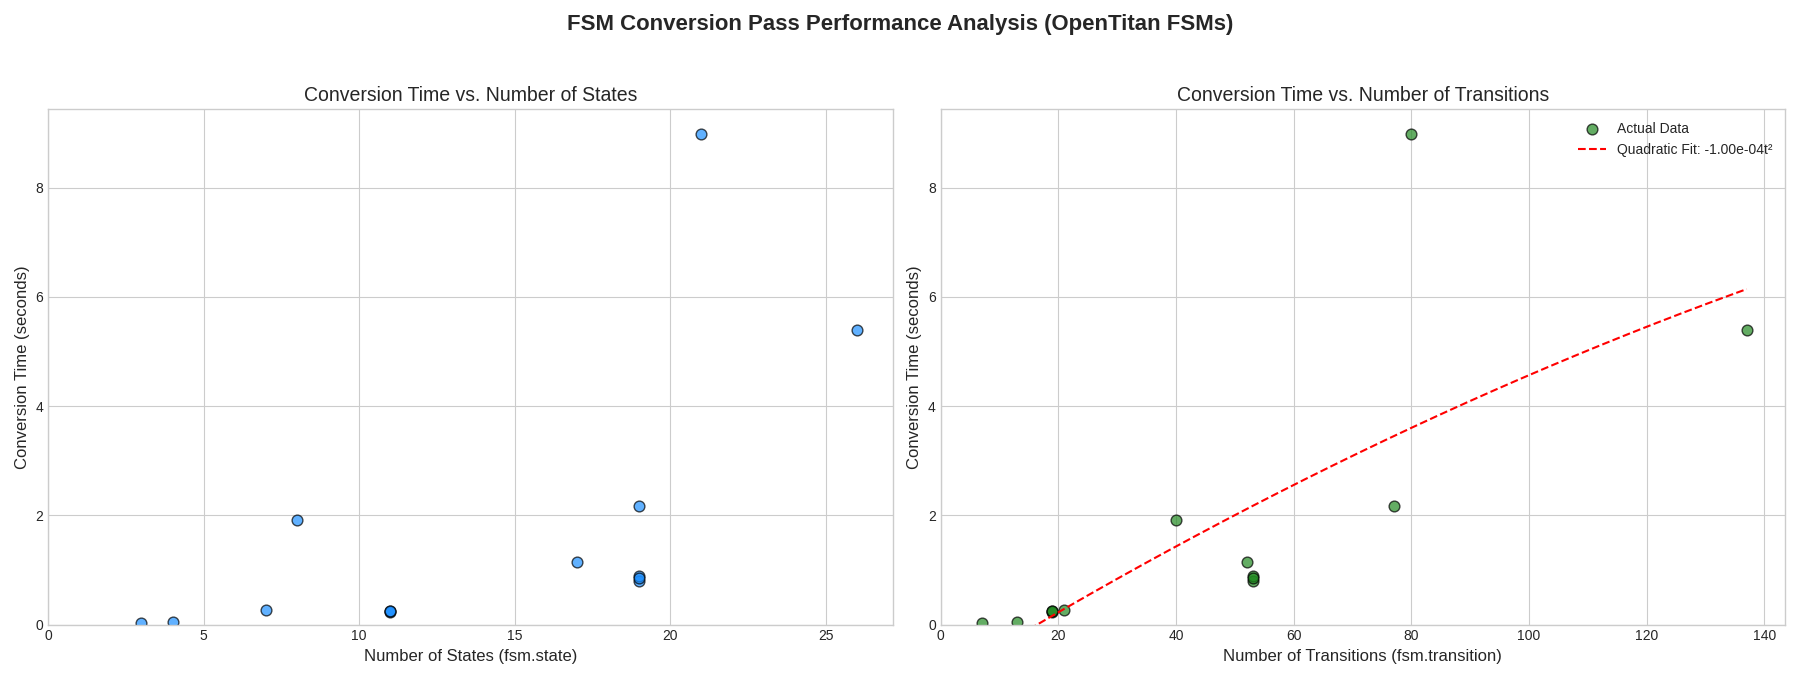
\includegraphics[width=\columnwidth]{fsm_conversion_performance_plot.png}

\caption{Performance of RTL-to-FSM extraction over number of transitions and number of states on real-world FSMs.}
\end{subfigure}
    \hfill
    \begin{subfigure}[t]{0.49\textwidth}
  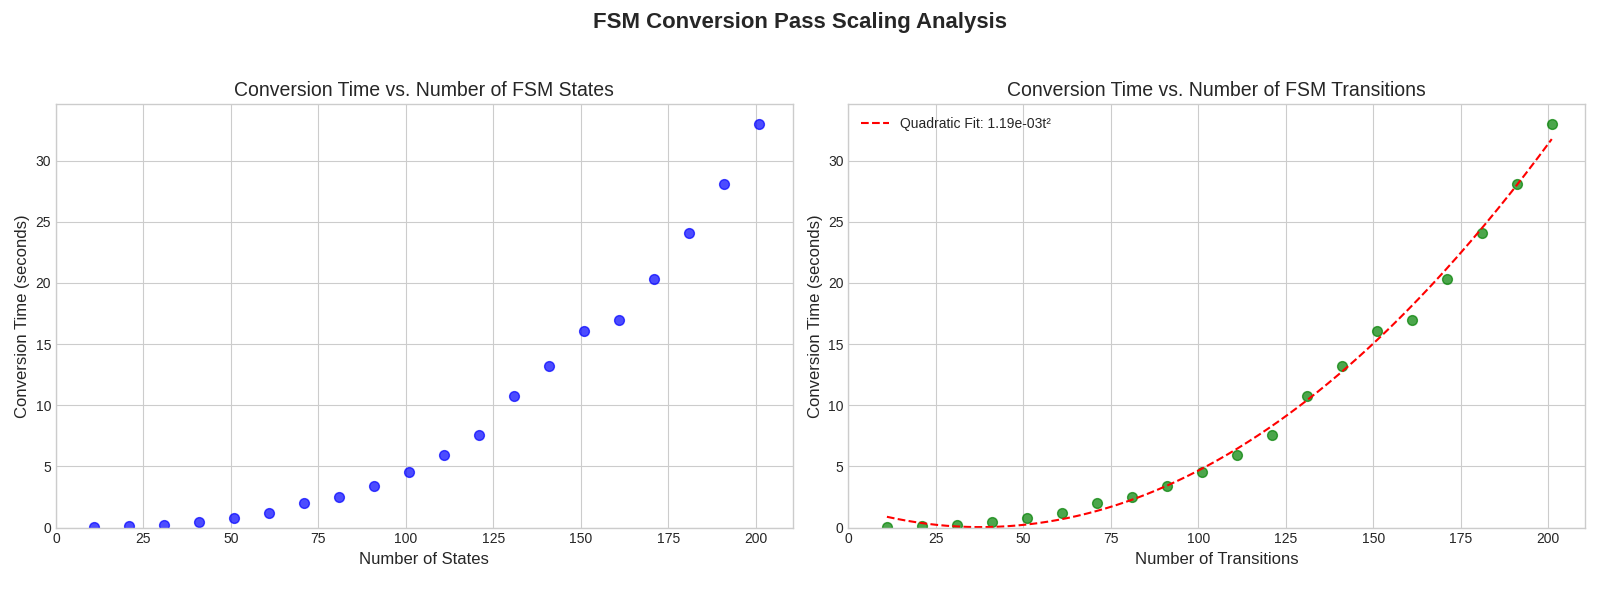
\includegraphics[width=\columnwidth]{fsm_conversion_scaling_plot.png}

\caption{Performance of RTL-to-FSM extraction over number of transitions and number of states on artificially constructed benchmark.}
\end{subfigure}

\caption{Performance of RTL-to-FSM extraction over number of transitions and number of states on artificially constructed benchmark and real-world FSMs.}
\label{fig:fsm-performance}
\end{figure*}

\begin{figure}
  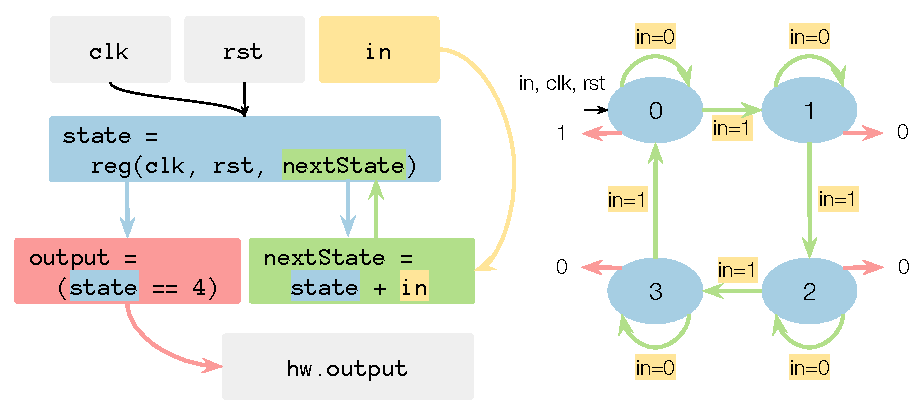
\includegraphics{rtl-to-fsm.pdf}
    \caption{When extracting an FSM from an RTL representation, 
      we map the circuit's functional units (on the left) to the states in the FSM (on the right). For a modulo-4 counter, 
      the RTL design contains an \textit{implicit} FSM composed of a state register, next-state logic, and output logic.
      To make this structure \textit{explicit}, we reify the four possible values of the state register into four distinct \texttt{fsm.state} operations, with the next-state and output logic distributed accordingly.}
    \label{fig:fsm-extraction}
\end{figure}


\begin{table*}[t]
\centering
\caption{FSM Conversion and Verification Summary on OpenTitan FSMs}
\label{tab:fsm_conversion}
\begin{tabular}{l S[table-format=4.0] S[table-format=3.0] S[table-format=1.4] l l}
\toprule
\textbf{FSM Name} & {\textbf{SV LoC}} & {\textbf{MLIR LoC}} & {\textbf{Time (s)}} & \textbf{Status} & \textbf{Details} \\
\midrule
adc\_ctrl\_fsm                   &  391 & 320 &  1.1521 & BMC Correct & OK \\
aes\_cipher\_control\_fsm         &  515 & 319 &  0.2647 & BMC Correct & OK \\
aes\_ctr\_fsm                    &  125 &  47 &  0.0234 & BMC Correct & OK \\
darjeeling\_pwrmgr\_fsm          &  566 & 353 &  0.8507 & BMC Correct & OK \\
darjeeling\_pwrmgr\_slow\_fsm     &  337 & 189 &  0.2297 & BMC Correct & OK \\
earlgrey\_pwrmgr\_fsm            &  560 & 355 &  0.8822 & BMC Correct & OK \\
earlgrey\_pwrmgr\_slow\_fsm       &  364 & 200 &  0.2427 & BMC Correct & OK \\
englishbreakfast\_pwrmgr\_fsm    &  721 & 347 &  0.8046 & BMC Correct & OK \\
englishbreakfast\_pwrmgr\_slow\_fsm &  364 & 200 &  0.2424 & BMC Correct & OK \\
i2c\_controller\_fsm             &  993 & 644 &  8.9873 & BMC Correct & OK \\
i2c\_target\_fsm                 & 1042 & 651 &  5.3982 & BMC Correct & OK \\
\textcolor{red}{lc\_ctrl\_fsm}   &  \textcolor{red}{890} & \textcolor{red}{342} &  \textcolor{red}{1.3648} & \textcolor{red}{CRASH}  & \textcolor{red}{circt-opt: fsm-to-core} \\
mbx\_fsm                        &  177 & 138 &  0.0538 & BMC Correct & OK \\
rom\_ctrl\_fsm                   &  358 & 227 &  2.1657 & BMC Correct & OK \\
spi\_host\_fsm.sv                &  645 & 393 &  1.9216 & BMC Correct & OK \\
\bottomrule
\end{tabular}
\end{table*}
%% \end{figure}

% \begin{figure*}[t]
%     \centering
%     % If you saved the compiled standalone PDF as "fsm_extraction_workflow.pdf"
%     % \includegraphics[width=\textwidth]{fsm_extraction_workflow.pdf}
%     \begin{tikzpicture}[
%     node distance=0.5cm and 1cm,
%     % Styles
%     process/.style={
%         rectangle,
%         rounded corners,
%         draw=blue!60!black,
%         fill=blue!10,
%         thick,
%         minimum height=1.2cm,
%         minimum width=3cm,
%         align=center,
%         font=\sffamily\bfseries
%     },
%     io/.style={
%         trapezium,
%         trapezium left angle=70,
%         trapezium right angle=110,
%         draw=green!60!black,
%         fill=green!15,
%         thick,
%         minimum height=1cm,
%         align=center,
%         font=\sffamily
%     },
%     codeblock/.style={
%         rectangle,
%         draw=gray!80,
%         fill=gray!10,
%         font=\small\ttfamily,
%         align=left,
%         rounded corners=3pt
%     },
%     tool/.style={
%         rectangle,
%         draw=orange!80!black,
%         fill=orange!20,
%         font=\sffamily\footnotesize,
%         rounded corners=2pt,
%         text=black
%     },
%    arrow/.style={
%         thick,
%         draw=black!70
%     },
%     dataflow/.style={
%         draw=black!50,
%         dashed
%     },
%     paneltitle/.style={
%         font=\sffamily\bfseries\Large,
%         text=black!80
%     },
% ]


% %======================================================================
% % Panel 1: FSM Extraction Algorithm
% %======================================================================

% % --- Nodes ---
% \node[io, minimum width=4cm] (inputrtl) {Input: `hw.module` \\ (Core Dialects)};

% \node[codeblock, below=0.5cm of inputrtl, text width=5cm] (inputcode) {
%     ...\\
%     \textcolor{red!70!black}{\%state\_q} = seq.compreg \textcolor{blue!70!black}{\%state\_d}, %clk \\
%     ... \\
%     \textcolor{blue!70!black}{\%state\_d} = comb.mux \%cond, \%s1, \%s0 \\
%     ...
% };

% \node[process, below=1cm of inputcode, minimum height=2cm] (reachability) {
%     1. Identify State Registers \\
%     (e.g., `seq.compreg` named "state") \\
%     \vspace{2mm}
%     2. Begin Reachability Analysis \\ (Worklist Algorithm from Initial State)
% };

% % Loop representation
% \node[rectangle, draw=blue!50, dashed, rounded corners, inner sep=0.5cm, fit=(reachability)] (loopfit) {};
% \node[above=0.1cm of loopfit.north, font=\sffamily\bfseries\color{blue!80}] {For each reachable state S\textsubscript{i}};


% \node[process, below=2cm of reachability, fill=blue!5, text width=6.5cm] (stategen) {
%     3. Generate `fsm.state @S\textsubscript{i}` Output Logic
% };

% \node[codeblock, below=0.3cm of stategen, text width=6cm] (stategencode) {
%     // Clone module body, then specialize: \\
%     // Replace state register read with its value in S\textsubscript{i}
%     \textcolor{red!70!black}{\%state\_q} = seq.compreg ... \\
%     \textbf{\huge $\Rrightarrow$} \\
%     \textcolor{red!70!black}{\%state\_q\_val} = hw.constant \textcolor{purple!80!black}{S\textsubscript{i}}
% };


% \node[process, right=0.5cm of stategen, fill=blue!5, text width=3.5cm] (transgen) {
%     4. Generate `fsm.transition @S\textsubscript{i} -> @S\textsubscript{j}` Guard Logic
% };

% \node[codeblock, below=0.3cm of transgen, text width=2.5cm] (transgencode) {
%     // In another clone, check if next-state logic \\
%     // evaluates to the value of a target state S\textsubscript{j}
%     \%is\_next\_state\_j = comb.icmp eq \textcolor{blue!70!black}{\%state\_d}, \\
%     \hspace{2.5cm} (hw.constant \textcolor{purple!80!black}{S\textsubscript{j}})
% };

% \node[io, below=2.5cm of stategencode, minimum width=4cm, fill=green!20] (outputfsm) {Output: `fsm.machine`};

% \node[codeblock, below=0.5cm of outputfsm, text width=5.5cm] (outputcode) {
%     fsm.machine @fsm(...) -> (...) \{ \\
%     \hspace{0.5cm}fsm.state @\textcolor{purple!80!black}{S\textsubscript{i}} \{ \\
%     \hspace{1cm} // Specialized output logic \\
%     \hspace{0.5cm}\} \\
%     \hspace{0.5cm}fsm.transition @\textcolor{purple!80!black}{S\textsubscript{j}} guard \{ \\
%     \hspace{1cm}fsm.return \%is\_next\_state\_j \\
%     \hspace{0.5cm}\} \\
%     \}
% };

% % --- Arrows ---
% \draw[arrow] (inputrtl) -- (inputcode);
% \draw[arrow] (inputcode) -- (reachability);
% \draw[arrow] (reachability) |- ($(reachability) + (0, -1)$) -| (stategen);
% \draw[arrow] (reachability) |- ($(reachability) + (0, -1)$) -| (transgen);
% \draw[arrow] (stategen) -- (stategencode);
% \draw[arrow] (transgen) -- (transgencode);
% \draw[arrow] (stategencode) -- ++(0,-0.5) -| (outputfsm);
% \draw[arrow] (transgencode) -- ++(0,-0.5) -| (outputfsm);
% \draw[arrow] (outputfsm) -- (outputcode);


% %======================================================================
% % Panel 2: Equivalence Checking Pipeline
% %======================================================================
% \begin{scope}[xshift=11cm, yshift=-3.5cm]

% % --- Nodes ---
% \node[io] (svin) {SystemVerilog FSM \\ (e.g., from OpenTitan)};

% \node[process, below=of svin] (ingest) {Ingest \& Pre-process};
% \node[tool, right=0.2cm of ingest, xshift=-0.5cm] (circt_verilog) {\texttt{circt-verilog}};

% \node[process, below=of ingest] (flatten) {Flatten to Golden Reference \\ (Core Dialects)};
% \node[tool, right=0.2cm of flatten, xshift=-0.5cm] (circt_opt1) {\texttt{circt-opt}};

% % Diverging paths
% \node[process, below=of flatten] (pass_test) {Apply Pass Under Test};
% \node[tool, left=0.2cm of pass_test, xshift=0.5cm] (pass_tool) {\texttt{--convert-core-to-fsm}};

% \node[process, below=of pass_test] (roundtrip) {Round-trip to Core Dialects};
% \node[tool, left=0.2cm of roundtrip, xshift=0.5cm] (rt_tool) {\texttt{--convert-fsm-to-core}};

% \node[process, below=4.5cm of flatten] (miter) {Generate Miter Circuit};

% % Miter internal diagram
% \begin{scope}[on background layer]
%     \node[rectangle, rounded corners, draw=purple!50, fill=purple!5, inner sep=0.5cm, fit=(miter)] (miterbg) {};
% \end{scope}

% \node[rectangle, draw, fill=white, minimum width=1.5cm, above right=-0.1cm and 0.4cm of miter] (mitergolden) {Golden};
% \node[rectangle, draw, fill=white, minimum width=1.5cm, below right=0.1cm and 0.4cm of miter] (miterdut) {DUT};
% \node[circle, draw, minimum size=0.5cm, right=1.2cm of miter.east, xshift=0.5cm] (miterxor) {$\oplus$};
% \node[rectangle, draw, fill=red!10, right=0.5cm of miterxor] (miterassert) {\texttt{assert}};

% % Final steps
% \node[process, below=of miter] (bmc) {Bounded Model Check};
% \node[tool, right=0.2cm of bmc, xshift=-0.5cm] (circt_bmc) {\texttt{circt-bmc}};

% \node[io, below=of bmc, fill=green!25] (pass) {Equivalent};
% \node[io, right=of pass, fill=red!25] (fail) {Counterexample};

% % --- Arrows ---
% \draw[arrow] (svin) -- (ingest);
% \draw[arrow] (ingest) -- node[midway, right, font=\footnotesize\ttfamily] {1\_initial.mlir} (flatten);

% % Golden path
% \draw[arrow] (flatten.south) -- ++(0,-0.5) -| node[pos=0.25, above, font=\footnotesize\ttfamily] {3\_flattened\_ref.mlir} (miter.west);

% % DUT path
% \draw[arrow] (flatten.south) -- (pass_test);
% \draw[arrow] (pass_test) -- node[midway, right, font=\footnotesize\ttfamily] {4\_fsm\_dialect.mlir} (roundtrip);
% \draw[arrow] (roundtrip.south) -- ++(0,-0.5) -| node[pos=0.25, below, font=\footnotesize\ttfamily] {5\_roundtrip\_core.mlir} (miter.west);

% % Miter internal arrows
% \draw[dataflow] ($(miter.east)+(0.2, 0.5)$) -- node[above, font=\tiny] {inputs} (mitergolden.west);
% \draw[dataflow] ($(miter.east)+(0.2, -0.5)$) -- (miterdut.west);
% \draw[dataflow] (mitergolden.east) -- (miterxor.north);
% \draw[dataflow] (miterdut.east) -- (miterxor.south);
% \draw[dataflow] (miterxor.east) -- (miterassert.west);

% % Final arrows
% \draw[arrow] (miter) -- node[midway, right, font=\footnotesize\ttfamily] {6\_miter.mlir} (bmc);
% \draw[arrow] (bmc) -- (pass);
% \draw[arrow] (bmc) -- (fail);

% \end{scope}

% %======================================================================
% % Panel Titles and Bounding Boxes
% %======================================================================
% \begin{scope}[on background layer]
%     % Panel 1
%     \node[rectangle, rounded corners, draw=black!30, fill=black!3, inner sep=1cm,
%           fit=(inputrtl) (outputcode) (transgencode)] (panel1box) {};
%     \node[paneltitle, above=0.3cm of panel1box.north] (panel1title) {FSM Extraction Algorithm (`--convert-core-to-fsm`)};

%     % Panel 2
%     \node[rectangle, rounded corners, draw=black!30, fill=black!3, inner sep=1cm,
%           fit=(svin) (pass) (fail) (miterassert)] (panel2box) {};
%     \node[paneltitle, anchor=center, yshift=0.3cm] at (panel2box.north) {Equivalence Checking Verification Pipeline};
% \end{scope}

% \end{tikzpicture}


%     \caption{
%         The FSM extraction pass algorithm and its formal verification pipeline.
%         \textbf{(Left Panel)} The algorithm identifies state registers in a hardware module defined by Core MLIR dialects. It performs a reachability analysis, starting from the initial state defined by register reset values. For each reachable state, it specializes a copy of the module's logic to generate the corresponding `fsm.state` output block and the `fsm.transition` guard conditions. This process transforms an implicit state machine in RTL into an explicit representation in the FSM dialect.
%         \textbf{(Right Panel)} The verification pipeline, orchestrated by the test script, establishes correctness via formal equivalence checking. A "golden reference" netlist is generated by flattening the input SystemVerilog. Concurrently, the pass under test (`--convert-core-to-fsm`) and its inverse (`--convert-fsm-to-core`) are applied to create a "design under test" (DUT). A \textit{miter circuit} is constructed to compare the outputs of the golden reference and the DUT on all inputs, asserting their equivalence. A Bounded Model Checker (`circt-bmc`) then attempts to find a counterexample that violates this assertion. The absence of a counterexample proves the pass is correct for the given FSM.
%     }\label{fig:fsm_extraction_workflow}
% \end{figure*}

\section{Evaluation}
\label{sec:eval}

%figure here lives in previous section (TV) so that it's in the right place

We evaluate the performance of \toolname{} at both RTL and FSM level over hardware designs from real-world systems, high-level synthesis tools and synthetic generators.
We find below that while \toolname{}'s RTL engine is not particularly competitive, complementing it with the FSM engine allows verification of FSM designs very quickly, scaling better than other tools on synthetic benchmarks and achieving a 35.8\% reduction in model checking time over state-of-the-art RTL model checkers.

\subsection{Experimental Setup}
All benchmarks were run on a Ryzen 16-core 9950X system with 128GB of memory and Z3 version 4.8.12.
We use the most recent versions (at the time of writing) of all mentioned tools for our evaluation\footnote{Commit hashes for the used tools are:
  b09305204 (ABC), 38a20b0 (AVR), 43dae91c (BtorMC), a1bb693 (btor2tools), 29aad20 (chctools), db344f8 (ric3)
}.
\grosser{Should we give the CIRCT commit hash?}
Experiments were run 10 times, and graphs show the mean execution time.
Since \toolname{} digests designs which are represented in CIRCT's IRs, we export these designs to standard formats for benchmarking against other tools.
The lowerings we use between representations are shown in \autoref{fig:eval-structure}.
We convert CIRCT IR to B\textsc{tor}2 using CIRCT's export pass, and transform B\textsc{tor}2 to AIGER using the btor2aiger tool from the btor2tools repository~\cite{btor2tools}.
None of these transformations took more than 2 seconds to finish.
\toolname{}'s FSM to SMT lowering was the slowest of these, primarily bottlenecked by CIRCT's SMTLIB export pass, which we expect to see become faster as it matures.

\begin{figure}[t]
  \centering
  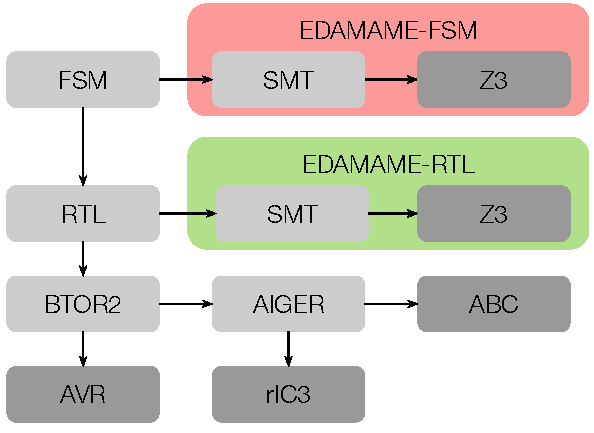
\includegraphics[width=\columnwidth]{methodology.pdf}
  \caption{We compare the performance of \toolname{}'s RTL engine against 1) AVR, after lowering the designs to B\textsc{tor}2 and 2) ABC and rIC3, after lowering the designs to AIGER.
           We compare the performance of \toolname{}'s FSM engine, which uses Z3, against AVR and rIC3.}
  \label{fig:eval-structure}
\end{figure}

\begin{table}[]
  \centering
  \small
  \caption{We use recent versions of all mentioned tools for our evaluation --- GitHub commit hashes are listed below.}
  \label{tab:commit-hashes}
  \begin{tabular}{cc}
    \toprule
    {\thead[t]{Tool}} & {\thead[t]{Commit Hash}} \\
    \midrule
    ABC          & b09305204 \\
    AVR          & 38a20b0 \\
    BtorMC       & 43dae91c \\
    btor2tools   & a1bb693 \\
    chctools     & 29aad20 \\
    rIC3         & db344f8 \\
    \end{tabular}
  \end{table}

\subsection{Evaluating \toolname{}'s RTL Engine}
\label{sec:bmc-eval}

We evaluate \toolname{}'s performance over RTL against three other BMC engines.
\begin{itemize}
  \item{The BMC engine of AVR~\cite{avr}}
  \item{BtorMC, the model checker published with B\textsc{tor}2~\cite{btor2}}
  \item{The BMC engine of ABC~\cite{abc}, a popular synthesis and verification tool}
\end{itemize}

Both AVR and ABC have a history of performing well in past HWMCCs, and a modified (but not publicly available version) of BtorMC has also placed well in the past.
We use three benchmarks to assess their performance:

\textbf{miter:} A very simple miter circuit that checks the equivalence of two circuits - one with a register on the output of an adder, the other with registers on the adder's inputs.
The property is that these circuits have equivalent outputs.

\textbf{fsm:} A 20-state counter FSM from the linear benchmarking suite
discussed below. Our model checkers check that in the final state, the counter variable is
always 20. We include only one FSM to avoid skewing our findings towards a specific structure.

\textbf{muldiv:} The multiplier/divider unit from the small configuration of the
Rocket RISC-V chip~\cite{ucb2016rocket}. Our model checkers check that if a non-overflowing multiplication was requested, the next output is the result of this multiplication.

\begin{figure}
  \centering
  \begin{subfigure}{\columnwidth}
  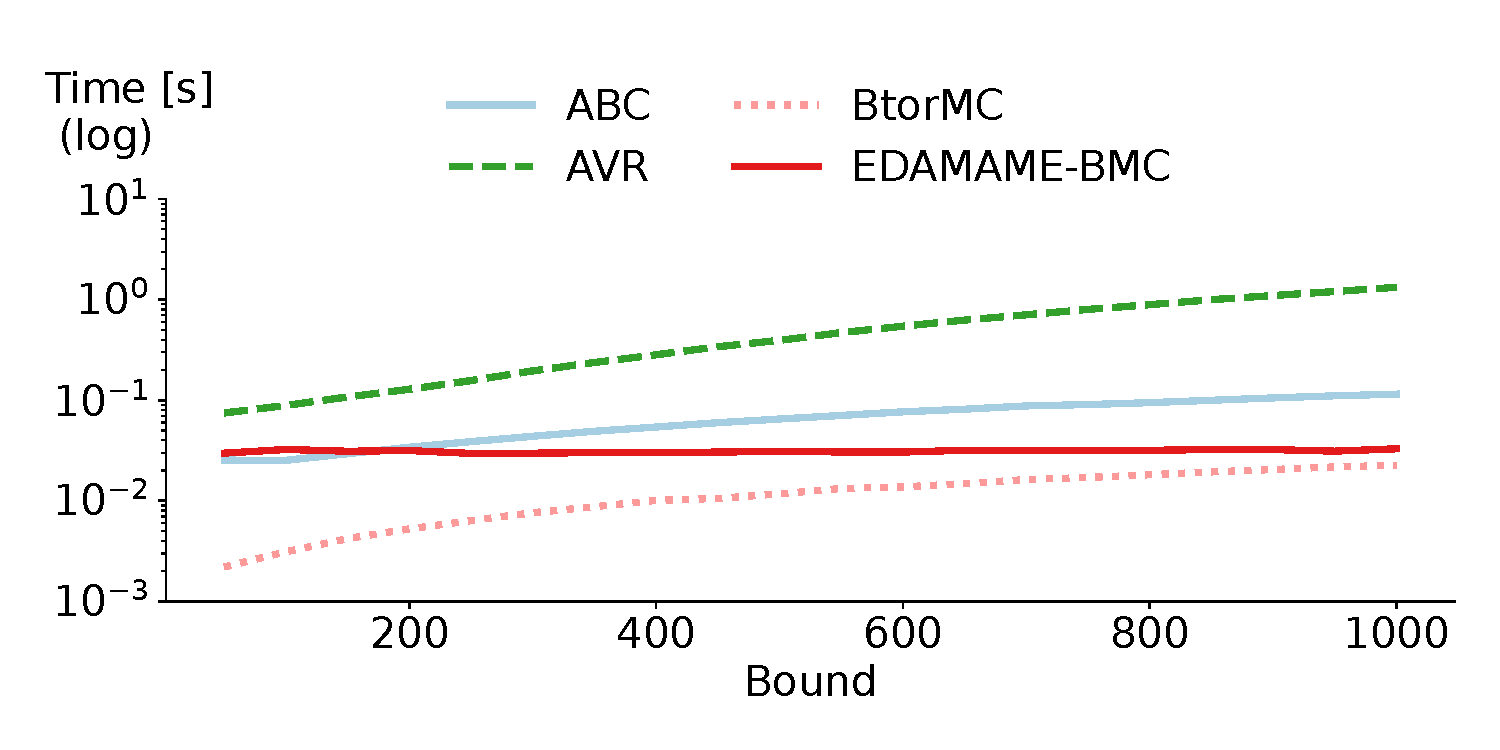
\includegraphics[width=\columnwidth]{bmc-plots/mitre.pdf}
  \subcaption[]{Time to model check \textbf{miter}.}\label{fig:benchmark-lin-s}
  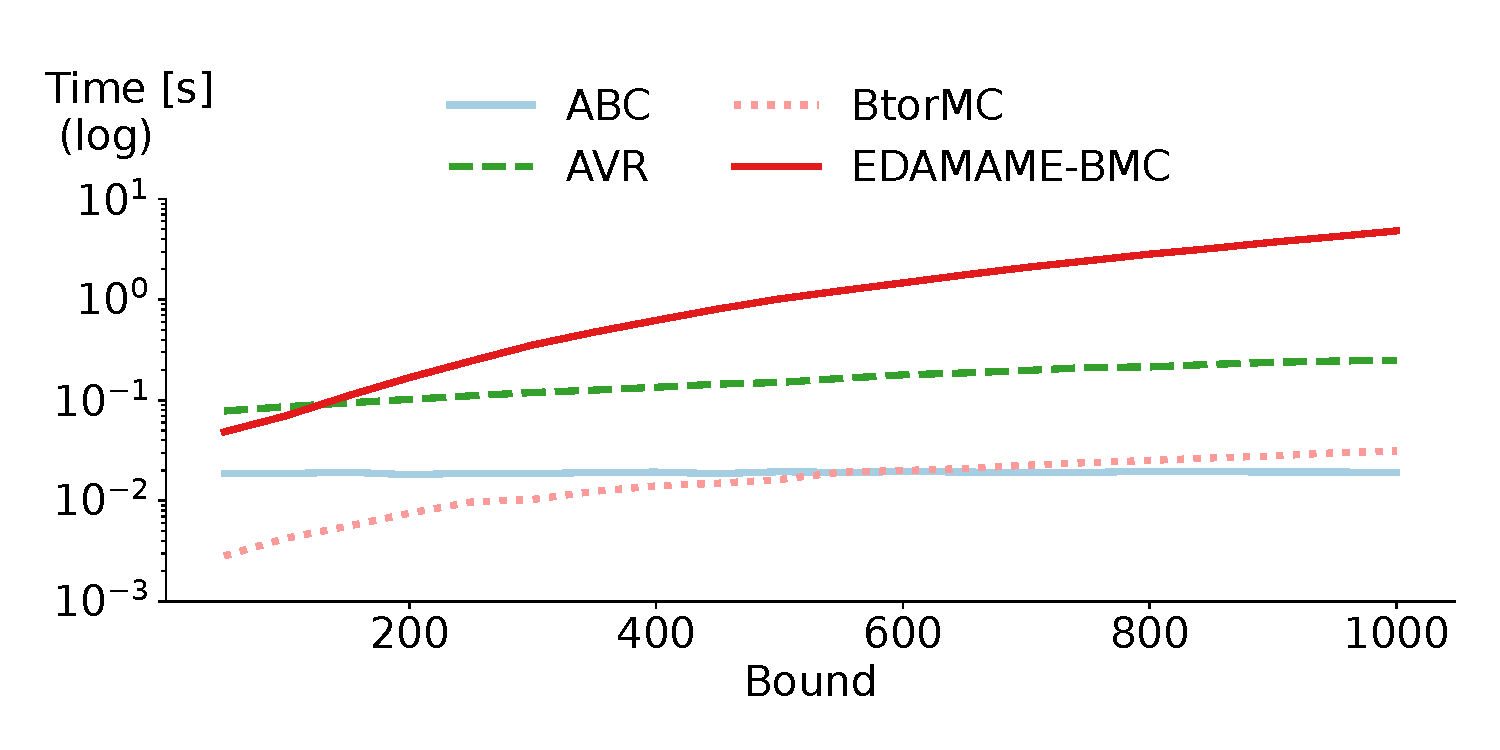
\includegraphics[width=\columnwidth]{bmc-plots/fsm.pdf}
  \subcaption[]{Time to model check \textbf{fsm}.}\label{fig:benchmark-lin-l}
  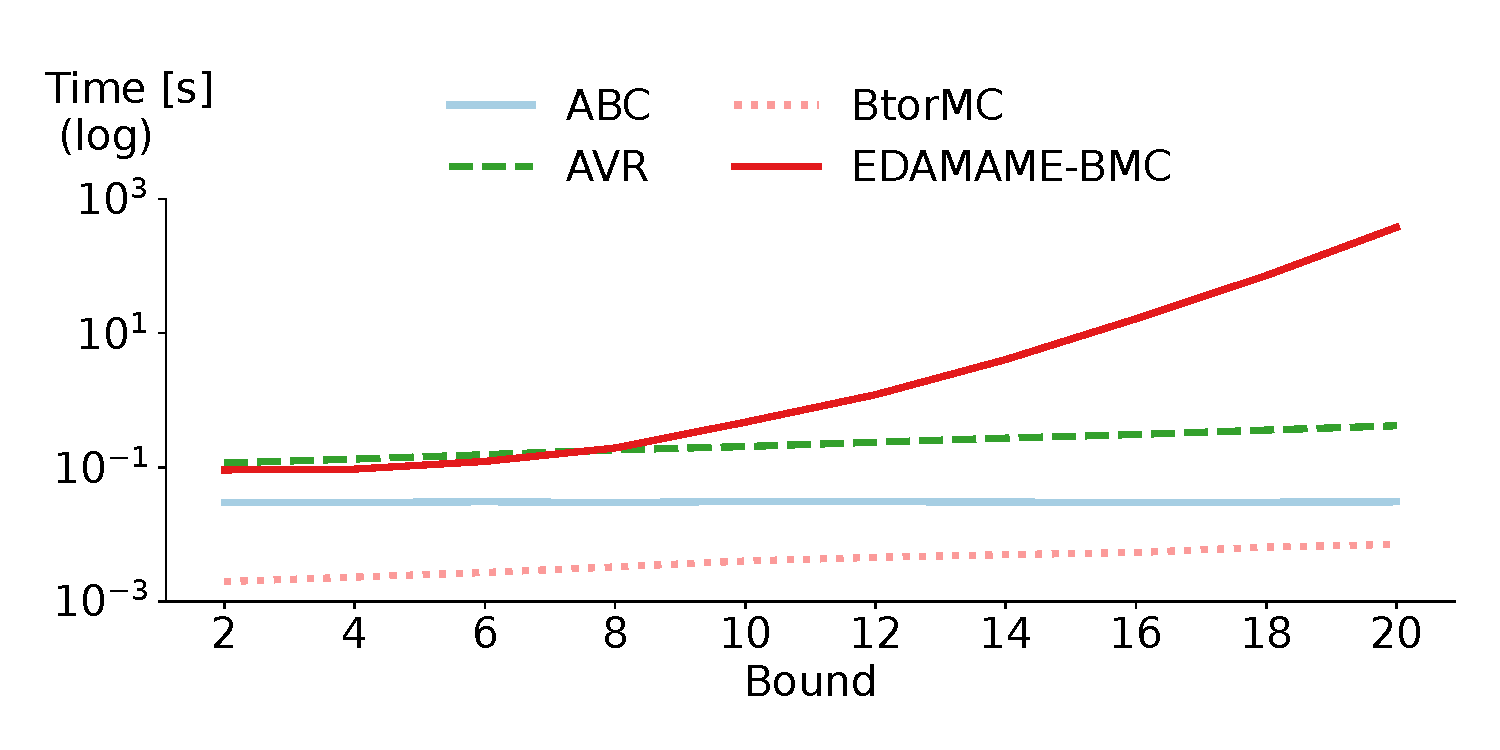
\includegraphics[width=\columnwidth]{bmc-plots/MulDiv.pdf}
  \subcaption[]{Time to model check \textbf{muldiv}.}\label{fig:benchmark-err-s}
\end{subfigure}
  \caption{\toolname{}'s RTL engine scales significantly worse than other BMC engines on non-trivial designs.}\label{fig:benchmark-bmc}
\end{figure}  

\arjun{It's important to acknowledge the fact that other tools are better in certain aspects. But  personally, if we're not competitive, then I don't think it's super important to evaluate in high detail exactly how uncompetitive we are. As a reader and potential user of your research, I'm not sure it helps me to see three different graphs showing how slow you are on each. It's enough for me to read a sentence or two explaining that SOTA BMCs scale better on fsm and muldiv, while EDAMAME scales very well (seemingly better than the competing solvers) on miter. I also think that none of this requires the amount of space that has been dedicated to introducing the competing BMCs.}
In \autoref{fig:benchmark-bmc} we compare the performance of each model checker over these benchmarks as the time bound increases.
\christos{IMHO, this is the point where the actual evaluation starts.}
We can see that, as expected, \toolname{}'s simple RTL engine is not very competitive with state-of-the-art, scaling significantly worse in runtime than the other model checkers.
Z3 is not specifically optimized for bitvector problems, and the RTL engine naively pops and pushes the portion of the circuit relevant to the property on each cycle without taking any advantage of incremental solving.
Z3 is the only SMT solver currently provided as a dependency of CIRCT, and this motivates dependencies on SMT solvers better optimized for the bitvector theories that hardware verification tooling tends to use.

\newpage
\subsection{Evaluating \toolname{}'s FSM Engine}

We wish not just to evaluate whether \toolname{}'s FSM engine is performant, but to determine whether introducing domain-specific algorithms provides a model checking time improvement that couldn't simply be achieved by implementing a particularly performant RTL model checking algorithm.
To this end, we benchmark \toolname{}'s FSM engine against two state-of-the-art RTL model checkers:

\begin{itemize}
  \item{AVR~\cite{avr}, the overall winner of the 2020 HWMCC (and second-place winner in 2024)}
  \item{rIC3~\cite{ric3}, the overall winner of the 2024 HWMCC}
\end{itemize}

These tools were both the winners by substantial margins at their respective HWMCCs, so are accurate indicators of the best performance \toolname{} could achieve just by implementing alternative RTL model checking algorithms.

\subsubsection{Benchmarks}

We benchmark on synthetic benchmarks to assess the scalability of \toolname{}'s approach and on real-world FSMs from open-source EDA projects and an HLS flow to verify that the approach is competitive on realistic hardware structures.

\begin{figure}[]
  \centering
  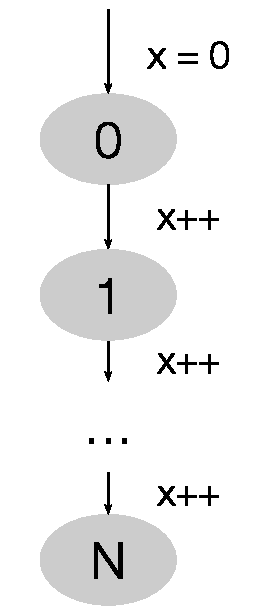
\includegraphics[width=0.3\columnwidth]{linear-struc.pdf}
  % \subcaption[Linear FSMs]{}\label{fig:benchmark-lin}
  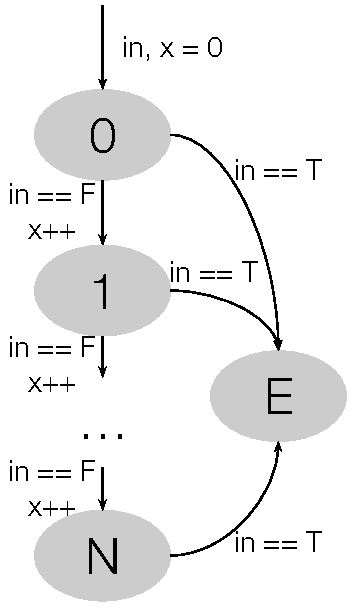
\includegraphics[width=0.38\columnwidth]{err-struc-vert.pdf}
  % \subcaption[Error-state FSMs]{}\label{fig:benchmark-err}
  \hfill
  \caption{We introduce two synthetic benchmarks sets to assess the scalability of our approach: 
  one comprising non-branching counting FSMs and one comprising FSMs with a single error state, 
  transitioned to when the input is true.} \label{fig:benchmark-struc}
\end{figure}

\paragraph{Synthetic FSMs for scaling analysis:}
\arjun{Here and in general in your evaluation, I feel like I want to skim it and understand key results in terms of hard numbers. But instead, everywhere I look I seem to find more details of experimental setup, explanations of baselines and benchmarks :) I would suggest frontloading key numbers everywhere in the beginnings of paragraphs/sections.}
To demonstrate scalability experimentally, we check properties over a range of simple, synthetically generated FSMs with increasing size. 

We generate two types of synthetic benchmarks, as detailed in \Cref{fig:benchmark-struc}, for FSMs with different structures: 
\begin{itemize}
  \item linear: \acp{fsm} representing a basic counter with no branching, no loops and a 
  single variable incremented every time a transition is taken
  \item error: \acp{fsm} with a linear path followed when the input is false, and a single 
  terminal error state that all states transition to when the input is true
\end{itemize}

\paragraph{Real-World FSMs:}
\label{rw-para}

\begin{table}[]
  \centering
  \small
  \caption{We evaluate our tool on a suite of FSMs from real-world EDA flows which vary in size and complexity.}
  \label{tab:real-world-fsms}
  \begin{tabularx}{\columnwidth}{@{\extracolsep{\fill}}l @{} S[table-format=3.0] @{} S[table-format=2.0] @{} S[table-format=2.0] @{} S[table-format=2.0] @{} S[table-format=2.0]}
      \toprule
      {\bfseries FSM}           & {\thead[t]{Transitions\\(\#)}} & {\thead[t]{States\\(\#)}} & {\thead[t]{Inputs\\(\#)}} & {\thead[t]{Variables\\(\#)}} & {\thead[t]{Outputs\\(\#)}} \\
    \midrule
    hls1          & 141   & 72  & 3   & 23  & 15  \\
    hls2          & 33    & 24  & 2   & 19  & 12  \\
    hls3          & 57    & 36  & 2   & 19  & 12  \\
    hls4          & 18    & 18  & 1   & 15  & 9   \\
    hls5          & 20    & 20  & 1   & 16  & 9   \\
    hls6          & 142   & 70  & 2   & 17  & 12  \\
    opentitan1    & 5     & 3   & 4   & 3   & 3   \\
    opentitan2    & 14    & 7   & 7   & 0   & 3   \\
    pulp1         & 32    & 16  & 1   & 0   & 7   \\
    \bottomrule
    \end{tabularx}
\arjun{maybe caption more like: We evaluate our tool on a benchmark suite of FSMs encompassing a wide variety of sizes and complexities.}
\end{table}  

While generated \acp{fsm} are useful for evaluating how our approaches scale, we also
wish to ensure that our techniques work well on hardware structures and
verification properties that appear in real-world engineering, something
difficult to emulate with generated \acp{fsm}.
For this, we use three sources of real-world \acp{fsm}:
\begin{itemize}
  \item Six FSMs from the SpecHLS flow~\cite{spechls}. These \acp{fsm} describe
  speculative execution units generated from a high-level specification
  \item Two \acp{fsm} from the OpenTitan project~\cite{opentitan}, an open-source yet industrial-strength 
  silicon root-of-trust that has seen great success in industry~\cite{opentitan_good}
  \item One \ac{fsm} from the PULP platform~\cite{conti2024pulp}, specifically from the RISC-V debug
  unit project
\end{itemize}

These FSMs are all translated into CIRCT's \texttt{fsm} representation from their respective source languages.
\autoref{tab:real-world-fsms} shows the size and complexity of these FSMs.

\subsubsection{Safety Property Verification}

On our synthetically-generated benchmarks we verify that
the value of the counter at the last state of the \ac{fsm} is as expected, i.e., 
$counter = K$, where $K$ is the expected counter value at that state. 
We deliberately check this property on the last state to ensure that the verification is 
non-trivial. 

On the real-world benchmarks we check properties specified within the design when possible, 
or otherwise formulate alternative non-trivial safety properties. 
In particular, for the SpecHLS \acp{fsm}, we verify that certain variables have expected values in certain states.
To ensure that checking these properties is not trivial, we verify them at states 
where multiple transitions converge. 

\begin{figure}[t]
  \centering
  \begin{subfigure}{\columnwidth}
  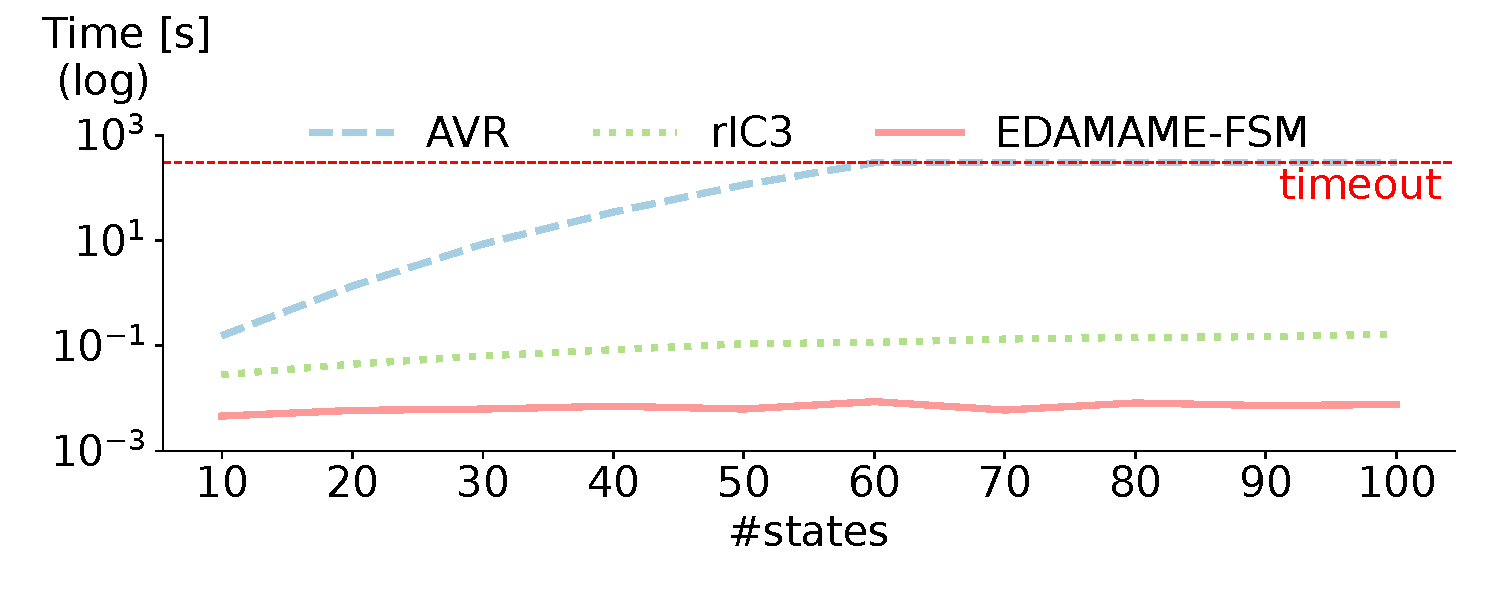
\includegraphics[width=\columnwidth]{fsm-plots/safety-sat_linear.pdf}
  \subcaption[]{Time to check safety properties on linear FSMs.}\label{fig:benchmark-lin-s}
  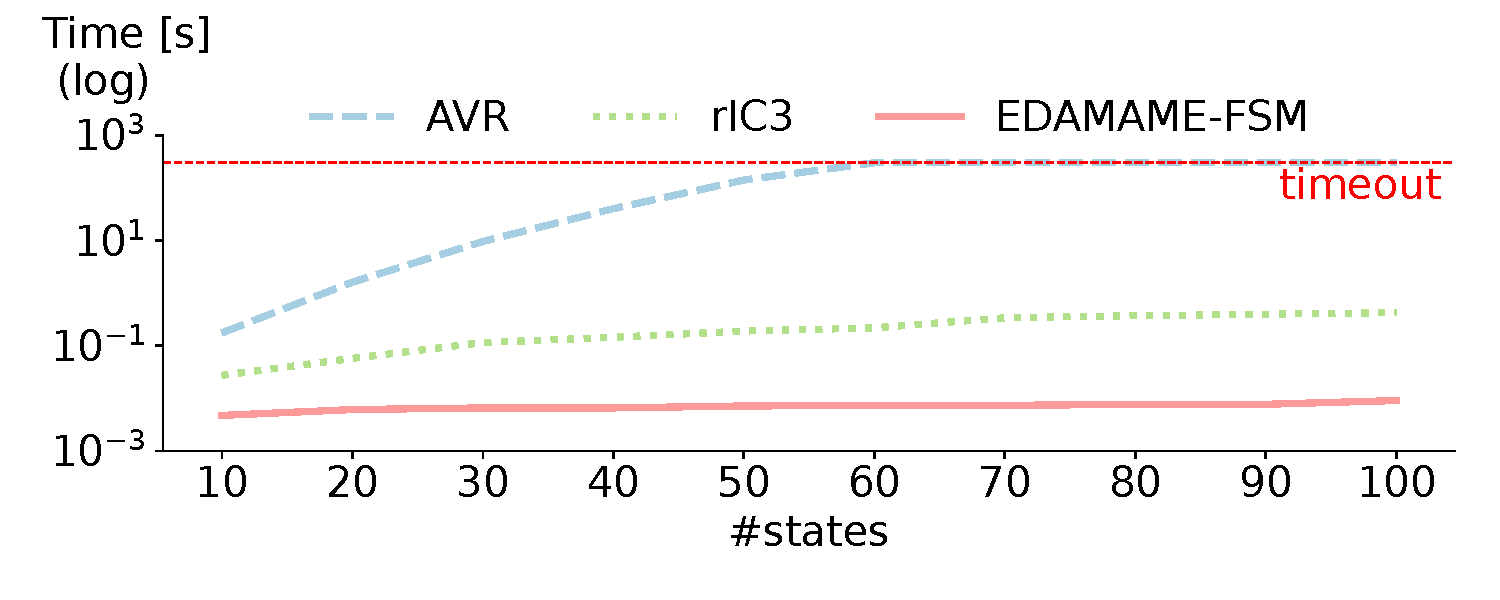
\includegraphics[width=\columnwidth]{fsm-plots/safety-sat_err.pdf}
  \subcaption[]{Time to check safety properties on err FSMs.}\label{fig:benchmark-err-s}
  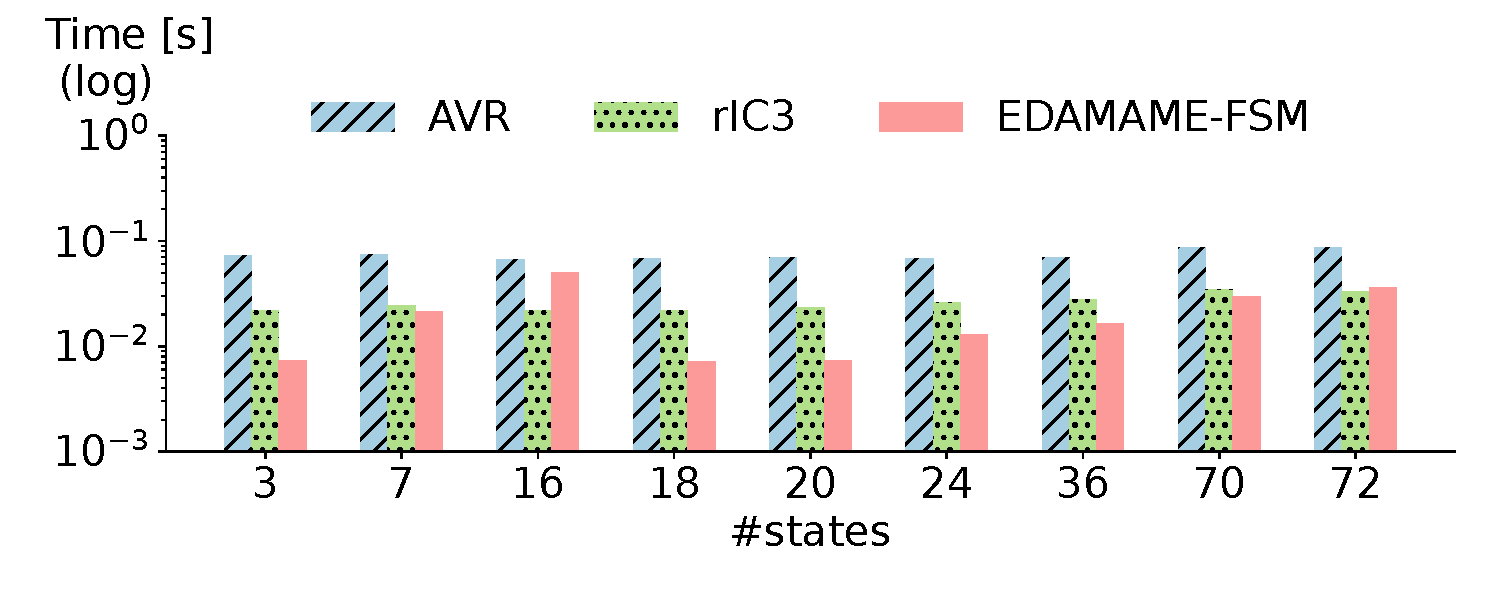
\includegraphics[width=\columnwidth]{fsm-plots/safety-sat_rw.pdf}
  \subcaption[]{Time to check safety properties on real-world FSMs.}\label{fig:benchmark-rw-s}
  \end{subfigure}
  \caption[]{\toolname{} is fast and scales well on safety properties that hold, 
    with a geomean time reduction of 92.7\%, 96\%, 35.8\% for linear, error and real-world benchmarks. Tools were run with a 5 minute timeout.}\label{fig:safety-results-sat}
  % \arjun{the TIMEOUT text is very angry >:(}
\end{figure}


\subsubsection{FSM Model Checking Results}
We display the time taken to model check safe safety properties (i.e., safety properties that hold) over our various benchmarks in \autoref{fig:safety-results-sat}.
\toolname{} and rIC3 both consistently outperform AVR, implying that AVR's syntax-abstraction guided approach to IC3 is not advantageous in the context of FSMs.
rIC3 is very performant, but varies significantly in runtime and is only faster than \toolname{} on two benchmarks.
\toolname{} is fast, with particularly strong scaling performance as the benchmarks grow.
On our real-world \acp{fsm}, \toolname{} achieves a geomean 35.8\% reduction in model checking time over rIC3.

\begin{figure}[t]
  \centering
  \begin{subfigure}{\columnwidth}
  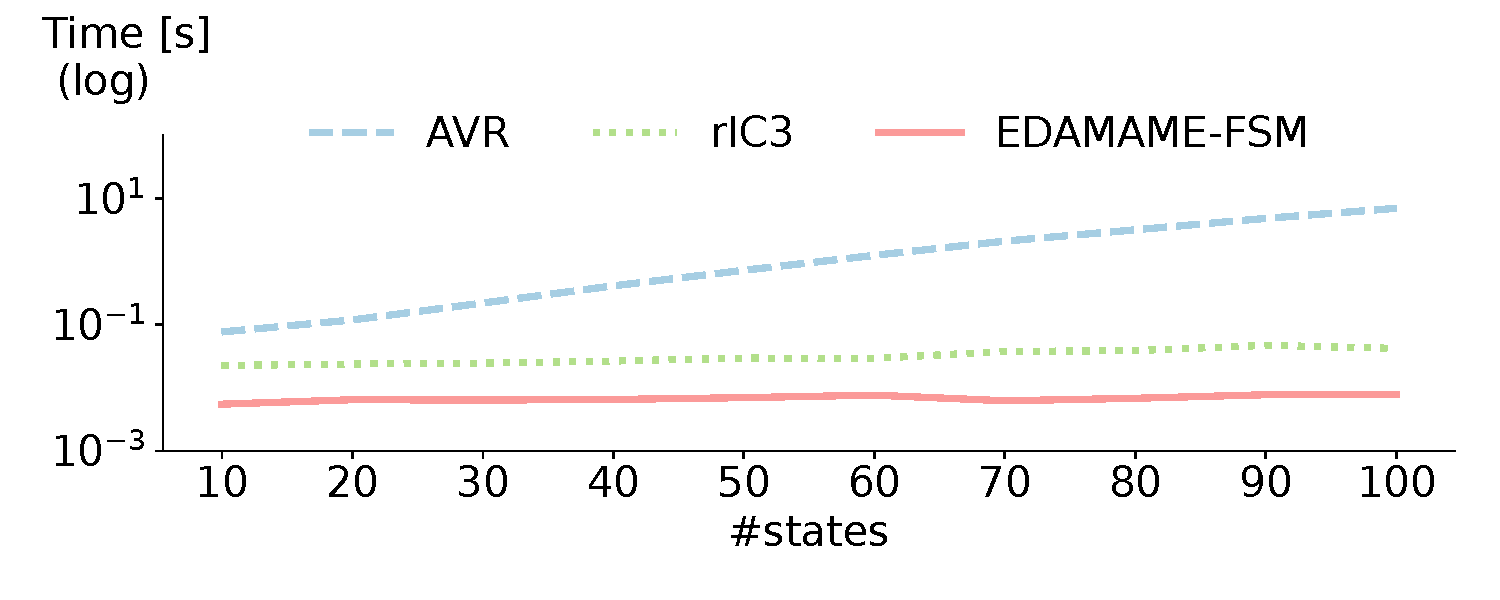
\includegraphics[width=\columnwidth]{fsm-plots/safety-unsat_linear.pdf}
  \subcaption[]{Time to check safety properties on linear FSMs.}\label{fig:benchmark-lin-s}
  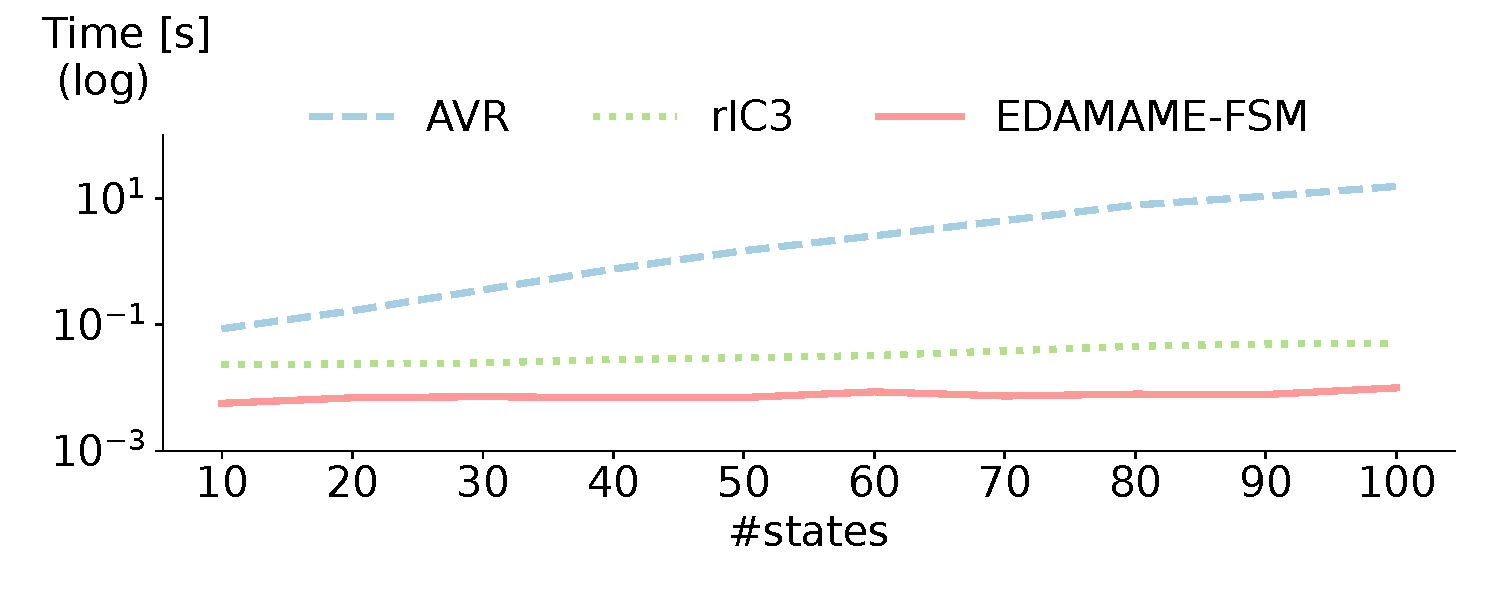
\includegraphics[width=\columnwidth]{fsm-plots/safety-unsat_err.pdf}
  \subcaption[]{Time to check safety properties on err FSMs.}\label{fig:benchmark-err-s}
  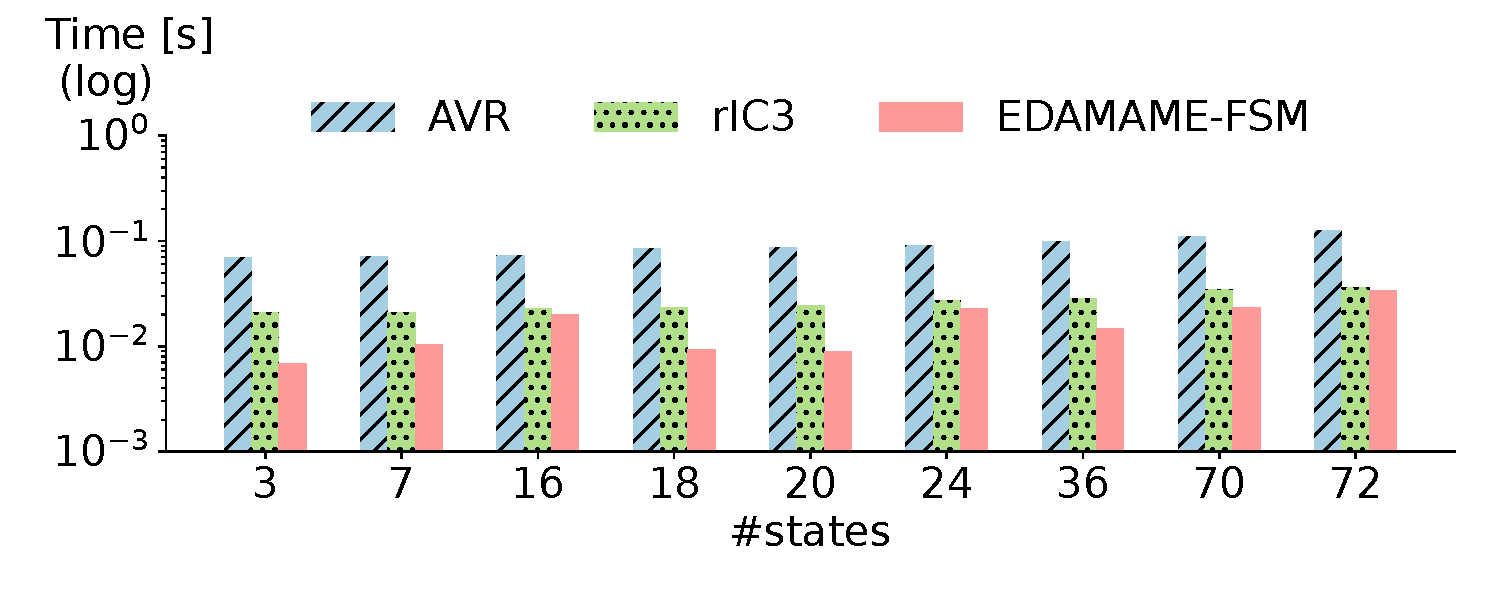
\includegraphics[width=\columnwidth]{fsm-plots/safety-unsat_rw.pdf}
  \subcaption[]{Time to check safety properties on real-world FSMs.}\label{fig:benchmark-rw-s}
  \end{subfigure}
  \caption[]{\toolname{} is fast to find that safety properties do not hold, as is rIC3. AVR, however, scales less well. \toolname{} reduces model checking time by 78.26\%, 77.4\% and 43.19\% (geomean) on linear, error and real-world benchmarks, respectively, over rIC3.
  }\label{fig:safety-results-unsat}
\christos{the legend is covering some of the plot lines; maybe use a single legend for this column of plots? I'd also flip the caption starting with our tool, because currently as it is phrased it seems to diminish our tool's lead in speed, while we have given so much real-estate to the above results?}
\end{figure}
% \healy{tops of these plots arecropped off}

Interestingly, we see on the 16-state PULP FSM that rIC3 significantly outperforms \toolname{} --- the only benchmark where this occurs by a large margin.
The FSM at hand is a JTAG state machine, and the property being checked is that the boolean outputs are mutually exclusive.
Because this is a combinational property over the FSMs outputs, rather than relating to one state, the property must be reiterated for every state in the FSM.
Thus, the FSM model contains several more assertions than the RTL model, which we expect to be the root of the slowdown --- indeed, only checking the state on one property is much faster.
This is unsurprising, as an RTL model checker needs only explore the multiplexer chains that feed into the outputs to check properties over them, while an FSM model checker must traverse the full transition system to confirm the property on each state.
Fortunately, \toolname{}'s architecture makes it easy for us to only use the FSM engine when it is advantageous.
We can simply add a catch or flag to fall back to the RTL model checker on properties that are not state-local (though it seems from our test suite that they tend to be state-local in practice).

In \autoref{fig:safety-results-unsat}, we check unsafe properties (i.e., properties that do not hold) on the same benchmarks to ensure that \toolname{}'s accelerated verification on safe properties does not come at the cost of a blowup on unsafe properties.
We see that \toolname{} is consistently the fastest to show that properties do not hold, with rIC3 also performing well.

\subsection{The Benefits of High-Level Structure}
\label{sec:chc-eval}

\begin{figure}[t]
  \centering
  \begin{subfigure}{\columnwidth}
  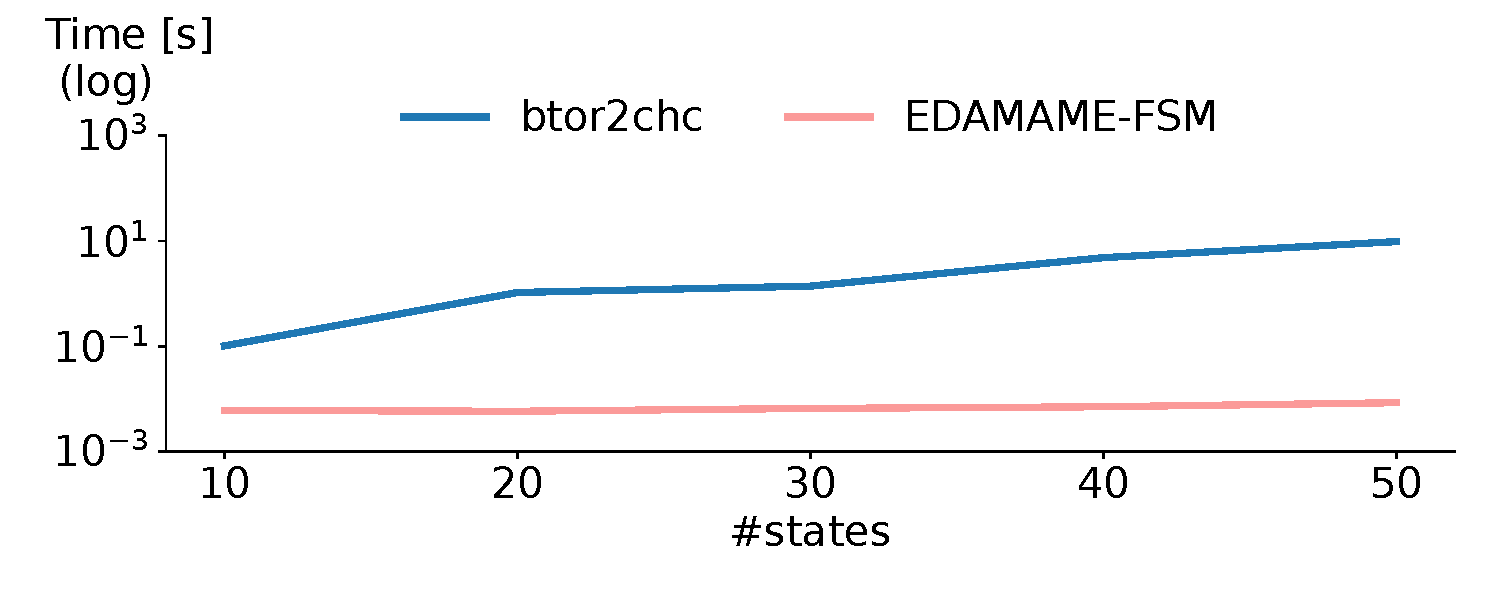
\includegraphics[width=\columnwidth]{chc-plots/safety-sat_chc_lin.pdf}
  \subcaption[]{Model checking time of linear FSMs with SPACER.}\label{fig:chc-lin}
  \end{subfigure}
  \begin{subfigure}{\columnwidth}
  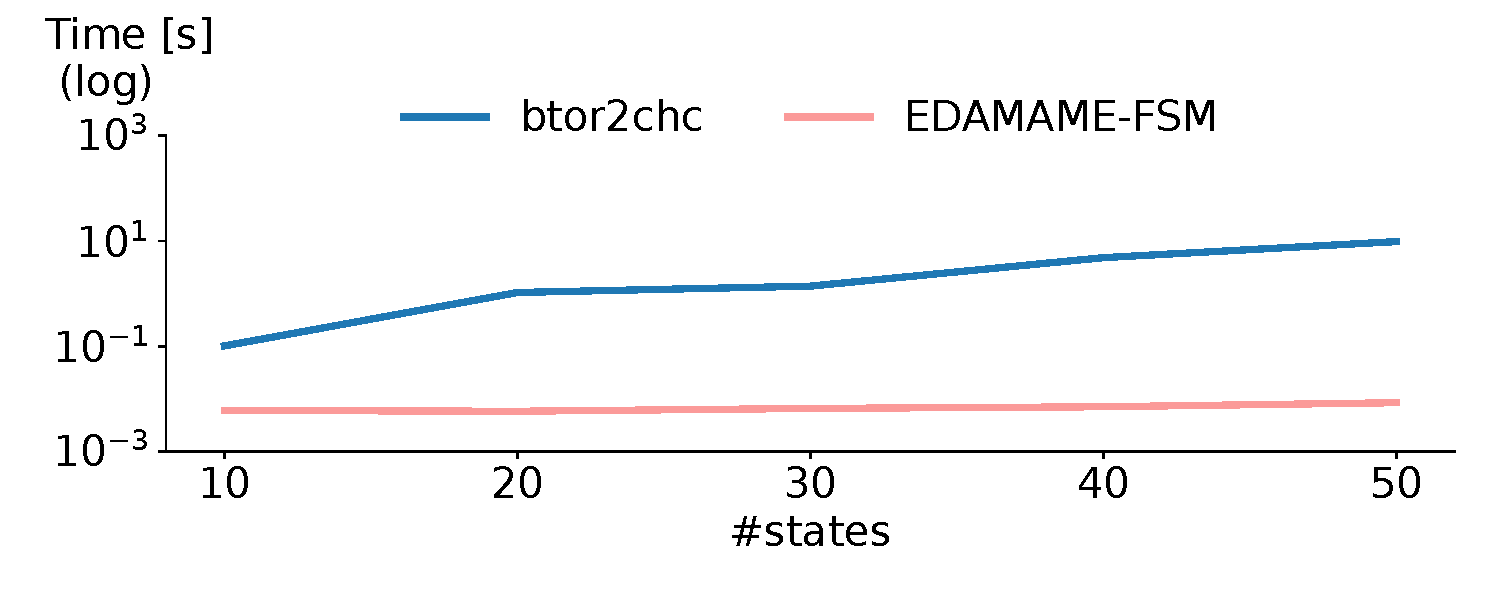
\includegraphics[width=\columnwidth]{chc-plots/safety-sat_chc_lin.pdf}
  \subcaption[]{Model checking time of error FSMs with SPACER.}\label{fig:chc-err}
  \end{subfigure}
  \begin{subfigure}{\columnwidth}
  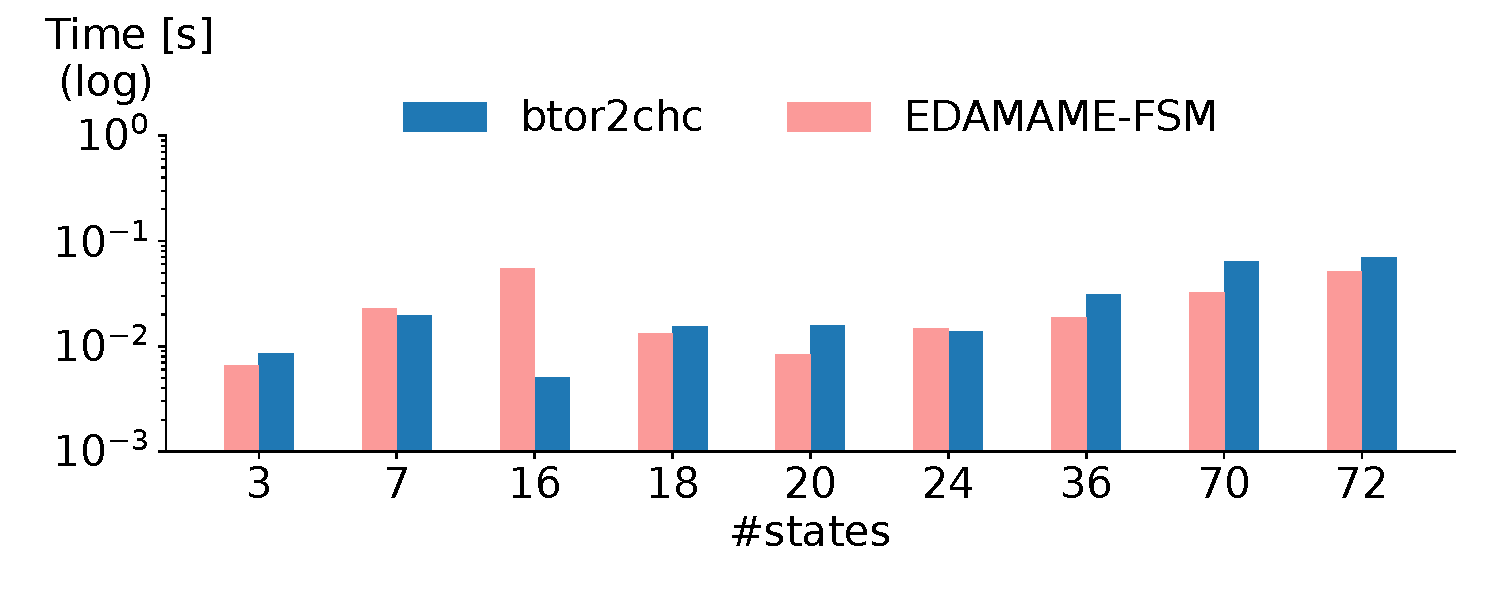
\includegraphics[width=\columnwidth]{chc-plots/safety-sat_chc_realworlds.pdf}
  \subcaption[]{Model checking time of real-world FSMs with SPACER.}\label{fig:chc-rw}
  \end{subfigure}
  \caption[]{SPACER's execution time over naively generated CHCs scales far faster than over the CHCs generated from a high-level FSM representation.
    Discarding the 16-state PULP \ac{fsm}, verifying CHCs generated from the \texttt{fsm} dialect reduces model checking time by 99.5\%, 99.5\% and 25.1\% (geomean) on 
    linear, error and real-world benchmarks respectively.
  }
  \label{fig:chc-comparison}
  \christos{maybe move the \toolname{}'s bar to the right, so it aligns with the legend order and the bar plot on the left column?}
\end{figure}
% \healy{missing benchmark to be added tomorrow (data is there, export script is just playing up)}

So far, we have seen that by using Z3's CHC solver engine SPACER, we can verify safety properties on the models of FSMs significantly faster than state-of-the-art tools.
However, with no baseline performance data for SPACER, it is unclear whether this is a result of the high-level structure \toolname{} extracts from the \texttt{fsm} dialect, or whether SPACER is simply an efficient engine that can solve these problems quickly regardless of this structure.
To provide a baseline for SPACER's performance, we use the btor2chc tool from the chctools repository~\cite{chctools}, a set of CHC tools provided by the organizers of CHC-Comp, a CHC solver competition.
This tool represents the entire circuit with just one invariant predicate, whose arguments describe the entire state of the circuit.
We use btor2chc to naively convert our benchmarks from RTL into CHCs, and then run SPACER on these CHCs.

\autoref{fig:chc-comparison} shows how long SPACER takes to check the Z3 files generated by \toolname{} compared to those generated naively by btor2chc.
We observe that \toolname{}'s models can be usually checked much faster, often by over an order of magnitude.
Furthermore, we note that in \autoref{fig:chc-lin} and \autoref{fig:chc-err}, the model checking time seems to scale significantly faster over btor2chc's output.
\toolname{}'s FSM engine is again slower, though, on the same 16 state PULP FSM, reinforcing the idea that \toolname{} performs best on state-local properties.

\newpage

\section{Related Work}
We briefly review how the work described here relates to work in related
EDA frameworks, exploiting abstractions for hardware
verification and model checking of state machines.

\subsection{Related Hardware Design and Verification Work}

K-CIRCT~\cite{zhao2024kcirct} provides a formal semantics for CIRCT's core dialects in the K framework.
K can then generate an RTL model checker and simulator automatically.
However, K-CIRCT does not explore higher-level dialects.

ChiselVerify~\cite{dobis2023chiselverify} is a hardware verification library for Chisel~\cite{bachrach2012chisel}, one of CIRCT's most widely-used front-end languages.
Among other contributions, it proposes formal methods for designs implemented in Chisel --- however, these are limited only to a single front-end and level of abstraction, while our approaches can generalize to any front-end.
% Need to expand with how it relates to our work

Yosys~\cite{yosys} is a widely-used and renowned open-source EDA toolchain, providing formal verification tooling through the SymbiYosys project~\cite{symbiyosys}.
However, SymbiYosys only operates on RTL designs stored in Yosys's internal representation.

\subsection{Using Abstractions for Hardware Verification}

Building high-level models of hardware that can be used for improved
verification procedures has been an ongoing area of research since at least as early as
1999~\cite{arvind1999trs}. BlueSpec SystemVerilog~\cite{bluespec} is arguably
the example of this that has seen the widest adoption, and has been integrated
with both SMT solvers~\cite{bluespec_smt} and interactive theorem
provers~\cite{bluespec_itp, koika}. The key advantage of our work over these approaches
is front-end neutrality and extensibility --- we can support any language
with a compiler that provides a lowering to CIRCT.

ILA~\cite{huang2018instruction} takes a similar approach to \toolname{} of building
a formal model from a high-level view of hardware, but focuses on
accelerators and their software interfaces.

CoSA~\cite{mattarei2018cosa} is a model-checking tool for the CoreIR hardware
IR~\cite{daly2018coreir}. CoreIR does not provide high-level abstractions, but
has a similar architecture to CIRCT, and CoSA is able to guide formal
verification using CoreIR-generated metadata. This approach may be applicable to
\toolname{}'s RTL engine, as the IRs operate at similar levels of abstraction.

Previous work has shown that using domain-specific information to directly guide
an SMT solver can improve its performance in program verification~\cite{chen2021leveraging}. This is a more fine-grained approach than ours, as
the SMT solver's decision procedures are guided on a per-program basis.
Extracting similar information may be possible from an FSM, which could further
improve performance over FSMs.

Vericert~\cite{herklotz2021vericert} addresses reliability issues in HLS toolchains by extending the verified CompCert C compiler~\cite{leroy2009compcert} to create a high-level synthesis flow mechanically proven to be correct.
Vericert solves a separate problem to \toolname{} (in that it verifies the correctness of the tooling itself, rather than designs) but uses an FSM-based intermediate language called HTL.
This may mean that the approaches used by \toolname{} could be used to accelerate the verification of hardware generated with Vericert.

% \paragraph{Using an SMT Solver for Checking the Completeness of FSM-Based Tests}
% This work~\cite{vinarskii2020using} will be useful in the generation of a testbench for our verification methodology. 
% The authors describe and formalize various properties related to \acp{fsm} description, to verify that a certain test set covers a set of cases. 
% This can also contribute to the motivations of our work, especially if we want to pursue a partitioning strategy. In fact, the authors argue that discarding \ac{fsm} details that are unnecessary to the property being checked is a good strategy

% \paragraph{Simulator independent coverage for RTL hardware languages}
% This work~\cite{laeufer2023simulator} deals with three issues in the context of coverage instrumentation and collection:
% \begin{itemize}
%     \item Most simulators lack support for collecting and reporting automated coverage metrics
%     \item Tools supporting these metrics exploit custom implementations, which make merging coverage across various software or simulators and formal tools difficult
%     \item Hardware languages do not usually support source-level coverage metrics
% \end{itemize}
% The authors present a new approach that exploits a compiler to lower coverage metrics to a single primitive that can be implemented for various simulators.
% Each compiler pass can introduce a metric. 
% This work is especially interesting because the authors also explore \ac{fsm} coverage, which can represent an interesting test case for our approach.
% \ac{fsm} coverage can represent an interesting use case for our approach, complementary to reachability analysis. 

\subsection{Model Checking State Machines}
Many program verification tools lower \acp{fsm} with safety properties to \acp{chc} with an approach similar to ours~\cite{bjorner2015horn}, including HSF~\cite{hsf} and SeaHorn~\cite{seahorn}.

Our lowering is not able to support liveness properties.
However, previous work has explored the conversion of liveness properties into safety properties~\cite{biere2002liveness, padon2017liveness} --- this would be a valuable addition to our work, allowing \toolname{} to support a new class of properties.

Previous works in ACL2~\cite{kaufmann1996acl2} have used decision procedures over \acp{fsm}~\cite{hunt2006sat} to verify hardware designs by representing an entire hardware design in finite-state automata form~\cite{hunt2017industrial}.
In particular, ACL2 compiles its internal SVEX representation, extracted from Verilog or SystemVerilog, into an \ac{fsm}.
However, this is an implicit representation of \acp{fsm} and mimics the structure of assignments seen in the SystemVerilog input, rather than explicitly outlining the structure as done in CIRCT's \texttt{fsm} dialect.

\section{Conclusion}
In an age where, more and more often, hardware has structural information directly encoded into its high-level representations, general-purpose model checking algorithms no longer make the most of the available information.
We propose complementing RTL model checking algorithms with domain-specific algorithms that verify over high-level abstractions, gaining performance without comprimising on generality.
We demonstrate this approach in \toolname{}, which combines a general RTL model checking algorithm with a dedicated algorithm for model checking FSMs to achieve substantial speedup over state-of-the-art when model checking FSMs.
Going forward, we hope to see more formal verification algorithms that can take advantage of the breadth of high-level abstractions available to us, demonstrating that a multi-level hardware compilation approach can be just as valuable to verification as it is to design.
\newpage

%   \cicolini{
%     Interesting refs:~\cite{witharana2022survey}: Hardware verification of modern
%     electronic systems has been identified as a major bottleneck due to the
%     increasing complexity and time-to-market constraints. One of the major
%     objectives in hardware verification is to drastically reduce the validation and
%     debug time without sacrificing the design quality. Assertion-based verification
%     is a promising avenue for efficient hardware validation and debug. In this
%     article, we provide a comprehensive survey of recent progress in assertion-based
%     hardware verification. Specifically, we outline how to define assertions using
%     temporal logic to specify expected behaviors in different abstraction levels.
%     Next, we describe state-of-the art approaches for automated generation of
%     assertions. We also discuss test generation techniques for activating assertions
%     to ensure that the generated assertions are valid. Finally, we present both
%     pre-silicon and post-silicon assertion-based validation approaches that utilize
%     simulation, formal methods as well as hybrid techniques. We conclude with a
%     discussion on utilizing assertions for verifying both functional and
%     non-functional requirements. Average project time spent in functional
%     verification. In 2020, the average verification effort is about 51\% of the
%     overall development effort (cost and time)~\cite{gupta1992formal}: We consider a
%     formal hardware verification problem to consist of formally estab- lishing that
%     an implementation satisfies a specification. The term implementation (Imp)
%     refers to the hardware design that is to be verified. This entity can correspond
%     to a design description at any level of the hardware abstraction hi- erarchy,
%     not just the final physical layout (as is traditionally regarded in some areas).
%     The term specification (Spec) refers to the property with respect to which
%     correctness is to be determined. It can be expressed in a variety of ways-as a
%     behavioral description, an abstracted structural description, a timing
%     requirement, etc. For the purpose of this survey, both entities-the
%     implementation and the specification-are regarded as given within the scope of
%     any one problem, and it is required to formally prove the appropriate
%     "satisfaction" relation. In particular, we do not address directly the problem
%     of specification validation, i.e. whether the specification means what it is
%     intended to mean, whether it really expresses the property one desires to
%     verify, whether it completely characterizes correct operation, etc. It can be
%     indirectly cast in terms of the formal verification framework described above in
%     the following sense-a specification for a particular verification problem can
%     itself be made the object of scrutiny, by serving as an implementation for
%     another verification problem at a conceptually higher level. The purpose of the
%     latter problem is to test if the meaning of the original specification is as
%     intended, the "intended" meaning thus serving as a specification at the higher
%     level. Note that this does imply a leap of faith at some level where
%     specifications are held to be infallible, a necessary characteristic of any
%     mechanism for formal representation. Similarly, at the lowest end as well, we do
%     not specifically address the problem of model validation, i.e. whether the model
%     used to represent the implementation is consistent, valid, correct etc. It is
%     obvious that the quality of verification can only be as good as quality of the
%     models~\cite{melham1988abstraction}: Recent advances in microelectronics have
%     given designers of digital hardware the potential to build electronic devices of
%     unprecedented size and complexity. With increasing size and complexity, however,
%     it becomes increasingly difficult to ensure that such systems will not
%     malfunction because of design errors. This problem has prompted some researchers
%     to look for a firm theoretical basis for correct design of hardware systems.
%     Mathematical methods have been developed to model the functional behaviour of
%     electronic devices and to verify, by formal proof, that their designs meet
%     rigorous specifications of intended behaviour. Proving the correctness of a
%     design using such hardware verification techniques typically involves: • Writing
%     a set of formulas S which express the specification of the device whose design
%     is to be proven correct. • Describing the design or implementation of the device
%     by a second set of formulas I. • Proving that a 'satisfaction' or correctness
%     relation holds between the sets of formulas I and S-i.e. that the implementation
%     satisfies the specifica- tion. This process is usually carried out at each level
%     of the structural hierarchy of the design. The top level specification is shown
%     to be satisfied by some connection of components; the specifications of these
%     components are in turn shown to be satisfied by their implementations, and so
%     on-until the level of primitive components is reached. If this technique is to
%     be used to verify large and complex designs, it is clear that the 'satisfaction
%     relation' that is used cannot be strict equivalence. Otherwise, at each level of
%     the design hierarchy, the specifications will contain all the information
%     present in the design descriptions at the level below. For large and complex
%     designs this means that the specifications at the upper levels of the hierarchy
%     will themselves become so large and complex that they can no longer be seen to
%     reflect the intended behaviour of the device. Furthermore, proofs of equivalence
%     between such complex formulas will become unmanageable, even when automated
%     theorem proving tools are used. A satisfaction or correctness relation based on
%     the idea of abstraction, rather than equivalence, is the key to making formal
%     verification of large designs tractable. The aim of this paper is to discuss the
%     role of abstraction in hardware verification and to show how various types of
%     abstraction can be formalised and used to control the complexity of
%     specifications and correctness proofs. The organisation of the paper is as
%     follows. Section 1 introduces the idea of abstraction and its role in
%     controlling the complexity of hardware verification. In section 2 an informal
%     description is given of four basic abstraction mechanisms that can be used in
%     proofs of hardware correctness. Section 3 contains a brief introduction to the
%     logic that will be used to prove devices correct, and reviews the standard
%     techniques for formally specifying the behaviour and structure of hardware in
%     logic. Sections 4 through 7 show how each of the four basic abstraction
%     mechanisms can be formalised in logic; in each section, an example is given to
%     illustrate the use of the abstraction mechanism being discussed.  
%     }













%   \section{Potential Storylines}
% \begin{itemize}
%   \item focus on circt-mc as a novel addition to circt, then introduce the idea
%   of model checking at higher abstraction levels (example: FSM, would be nice to
%   add another one) and potentially checking hybrid properties during the
%   lowering
% \end{itemize}

% \section{Weaknessess}
% \begin{itemize}
%   \item what's the purpose of verifying at high level if the lowering is not
%   guaranteed/verified?
% \end{itemize}

% \section{Takeaways and Ideas}

% \begin{itemize}
%     \item Checking FSMs is useful and there are various works dealing with it. 
%     \item Using an \ac{smt}-based approach takes time. \Cref{fig:t-scal} can be
%       a good motivation for optimizing the naive approach, e.g. by partitioning
%       the \ac{fsm} or using a hierarchical model. I would also like to try
%       checking each partition singularly and putting it all together.
%       Partitioning (e.g. exploiting graphs algorithms) sounds exciting, and we
%       could derive some partitioning algorithms that take into account the
%       property being checked. However, we must be careful not to play around
%       with logic assumptions too much (and we should probably ask Alex, too).
%     \item We could also consider partitioning the time, i.e., checking a small
%     set of time blocks at a time speculating on different starting
%     configurations for each set of blocks. In this case, we would then put it
%     all together, but again we must be careful from a logic perspective.
%     \item This \ac{fsm}-based approach can be useful for verifying \acp{fsm}
%     transformations (cfr. Gorius' work on speculative hardware). However, I
%     would say that running the actual \ac{fsm} is in general much easier for
%     this kind of comparison, so we should reason about an use case where doing
%     so is impossible.
%     \item Another interesting direction is the composition of \acp{fsm}, which
%     should be complementary to hierarchical automata (e.g. synchronous product).
% \end{itemize}

% \section{Introduction}

% Of this super cool article \ldots
% \grosser{A simple comment refering to a particular location}

% % If there is \authorTwo[some text we want to refer to specifically]{this looks
% % particularly interesting} we can refer to this text from within our comments.

% % And here we only mark \authorTwo[text]{} that is \authorTwo[interesting]{}, but do not
% % actually comment.

% Now we have a sequence of comments,
% % \authorThree{Comment 3}
% % \authorFour{Comment 4}
% % \authorFive{Comment 5}
% % \authorSix{Comment 6}
% which should not introduce overlong white space sequences.

% Sometimes it is also important to \emph{emphasize} text to understand if it is
% underlined or printed in italic.

% We sometimes use macros to state that a tool as the name \toolname{}{} in a
% flexible way.

% \lipsum[1-3]

% \begin{figure}
% % Link to figure
% %
% % https://docs.google.com/drawings/d/1juKp43D3rLC-luBQPwQZ_wCnDK2S_6C1k6USV0wKE0g/edit?usp=sharing
% \includegraphics[width=\columnwidth]{overview.pdf}
% \caption{Our key idea visualized}
% \grosser{Replace this figure with your own drawing.}
% \end{figure}

% \vspace{.5em}
% \noindent
% Our contributions are:
% \grosser{Always state your contributions explicitly: (A) this makes it
% easy for the reader to understand what novelty is presented, and (B)
% these contributions help you to focus. In particular, the objective of
% the remaining paper should be to support the claims stated here.
% }
% \begin{itemize}
% 	\item Contribution 1 (\autoref{sec:implementation})
% 	\item Contribution 2
% 	\item Contribution 3
% 	\item Contribution 4
% \end{itemize}

% \section{Our New Idea}

% \lipsum[1-3]

% \section{Implementation}
% \label{sec:implementation}

% \section{Related Work}

% \lipsum[1-3]

% \grosser{Related work should always be at the end of the document,
%          as it otherwise becomes an obstacle your reader must
% 	 overcome before reaching your idea. For details see:
% 	 \url{https://www.microsoft.com/en-us/research/academic-program/write-great-research-paper/}
% }

% \section{Conclusion}
% \lipsum[1]

% %% Acknowledgments
% \begin{acks}                            %% acks environment is optional
%                                         %% contents suppressed with 'anonymous'
%   %% Commands \grantsponsor{<sponsorID>}{<name>}{<url>} and
%   %% \grantnum[<url>]{<sponsorID>}{<number>} should be used to
%   %% acknowledge financial support and will be used by metadata
%   %% extraction tools.
%   This material is based upon work supported by the
%   \grantsponsor{GS100000001}{National Science
%     Foundation}{http://dx.doi.org/10.13039/100000001} under Grant
%   No.~\grantnum{GS100000001}{nnnnnnn} and Grant
%   No.~\grantnum{GS100000001}{mmmmmmm}.  Any opinions, findings, and
%   conclusions or recommendations expressed in this material are those
%   of the author and do not necessarily reflect the views of the
%   National Science Foundation.
% \end{acks}

% %% Bibliography
\bibliography{references}

% %% Appendix
% % Move \cleardouble and \appendix out of `draftonly` if you are using the
% % appendix
% \begin{draftonly}
% \cleardoublepage
% \appendix
% \section{Formatting and Writing Guidelines}

% These formatting guidelines aim to standardize our writing. They ensure that
% papers with multiple authors have a consistent look and that commonly occurring
% items are formatted in ways that are known to work well.

% \subsection{Figures}
% \label{appendix:figures}

% \paragraph{Referencing Figures} When referencing figures from the text we
% ensure the following:
% \begin{description}
%       \item [All figures are referenced] A paper with un-referenced figures appears incomplete.
%         We can check this using the \texttt{refcheck} package.
%         Issuing \texttt{make refcheck} on the commandline lists all \emph{labeled} elements that are not referenced in the text.
%       \item [References to figures are brief and easy to skip]~\\
%                 We minimize the number of words needed to refer to a figure. Reducing
%                 the number of non-information-carrying words directly increases
% 		the density of interesting content. When skipping references
% 		becomes easy, reading quickly while ignoring figures remains a
% 		smooth experience. The best and briefest reference to a figure
% 		is a link in parenthesis that is added after the subject
% 		representing the content depicted in a figure:\\
% 		{\color{pairedTwoDarkBlue}\textit{Figure
% 		X shows the design of A, which consists of ...}}\\
% 		$\to$ {\color{pairedFourDarkGreen}
% 		\textit{The design of A (Figure X) consists of ...}}
%       \item [The text is always self-contained without figures] ~\\ The reader
%                 should be able to read the text without ever looking at any
%                 figure. They should still understand the text and get the key
% 		message of each figure directly from the text. By not forcing
% 		the reader to analyze a figure while reading, we increase
% 		readability as the reader can continue reading without having
% 		to skip between text and figures. Such writing style also helps
% 		to guide the thoughts of the reader, who can (for a moment)
% 		trust our summary of the figure and does not need to develop
% 		their own interpretation on-the-fly, a task which often yields
% 		results that do not fit the flow of our exposition. Readers
% 		typically only feel that their reading is interrupted if there
% 		is no explanation of a figure at all. Hence, we do not need to
% 		discuss all details of a figure, but half a sentence that explains the
% 		core idea is typically sufficient for a reader to continue
% 		reading.  By making
% 		our text self-contained even when ignoring figures the reader
% 		experiences a smooth and uninterrupted reading experience.\\
% 		{\color{pairedTwoDarkBlue}
% 		\textit{The speedups are presented in Figure X. < a new topic> }}\\
% 		$\to$ {\color{pairedFourDarkGreen}\textit{Our approach outperforms the state of the art
% 		XXX-library (Figure 3) demonstrating more than 4x speedup on
% 		test case 1 and 2 and a geometric mean speedup of 1.5x over all
% 		20 test cases.}}
% \end{description}
% We reference figures in text using
% \texttt{\symbol{92}autoref\{fig:speedup\}} for a figure with label
% \texttt{fig:speedup}.  The use of autoref ensures that all references
% to figures are formatted consistently, e.g. as \autoref{fig:speedup}.

% \paragraph{Color Scheme} 

% In Figures we use a color scheme that is print-friendly and also visible
% with red-green blindness. The following colors are all print-friendly
% and red-green save when only using Color 1-4:

% \medskip
% {
% 	\small
% \newcolumntype{a}{>{\columncolor{pairedOneLightBlue}}c}
% \newcolumntype{b}{>{\columncolor{pairedTwoDarkBlue}}c}
% \newcolumntype{d}{>{\columncolor{pairedThreeLightGreen}}c}
% \newcolumntype{e}{>{\columncolor{pairedFourDarkGreen}}c}
% \newcolumntype{f}{>{\columncolor{pairedFiveLightRed}}c}
% \newcolumntype{g}{>{\columncolor{pairedSixDarkRed}}c}

% \begin{tabular}{a b d e f g}
% Color 1 & Color 2 & Color 3 & Color 4 & Color 5 & Color 6\\
% \#a6cee3 & \#1f78b4 & \#b2df8a & \#33a02c & \#fb9a99 & \#e31a1c
% \end{tabular}
% }

% We de-emphasize components in figures by using additionally two shades of gray.
% Especially in complex figures, it is often helpful to de-emphasize visual
% elements that we want to represent but that should not be the focus of a
% reader's attention.

% \medskip
% {
% 	\small
% \newcolumntype{h}{>{\columncolor{pairedNegOneLightGray}}c}
% \newcolumntype{i}{>{\columncolor{pairedNegTwoDarkGray}}c}

% \begin{tabular}{h i}
% Color -1 & Color -2\\
% \#cacaca & \#827b7b\\
% \end{tabular}
% }

% Single-color graphs are plotted in Color 1 --- Light Blue.

% \paragraph{Labels in Figures}
% Complex diagrams often benefit from labels inside the diagrams. We suggest to
% use a filled circle (e.g, in light blue) to highlight these numbers and use
% these references, e.g., \circled{1} implemented as \texttt{\textbackslash{}circled\{1\}}, in the text to refer to them.

% \paragraph{Captions and Core Message}
% \label{appendix:captions}

% Each figure should have a caption that makes a clear statement about this
% figure, as such a statement makes it easier for the reader to (in)validate the
% figure as evidence for the claim we make. Traditionally, figures often have a
% caption indicating its content:\\ {\color{pairedTwoDarkBlue} \textit{$\cdot$
% Speedup of approach A vs approach B on system X}}\\ {\color{pairedTwoDarkBlue}
% \textit{$\cdot$ Architecture diagram of our solution}}\\ While these statements
% clearly state the content of a figure at the meta-level, they often lack
% information about the precise content and the claim a figure is meant to
% evidence. While knowing that a figure is an architecture diagram is useful for
% the reader when looking at the figure the reader automatically asks two
% questions: (a) what properties set this architecture apart and (b) does its
% implementation deliver the claimed properties? Or, in more general terms, what
% claims do we aim to evidence with this figure and does the figure provide the
% needed evidence to support our claims? In theory, this information could be
% contained in the text of the paper, but to optimize for readers who skim the
% figures first, we want to offer them as part of the caption. Nevertheless, it
% makes often sense to word the caption strategically to still document the
% meta-level content of a figure.\\ $\to$ {\color{pairedFourDarkGreen}
% \textit{$\cdot$ Approach A is consistently faster than approach B, except for
% inputs that are not used in practice}}\\ $\to$ {\color{pairedFourDarkGreen}
% \textit{$\cdot$ The architecture of our design increases reusability by making
% components A, B, \& C independent of the core.}} For example, after reading the
% last caption the reader can validate if the architecture design indeed enables
% the promised independence, and we can double-check while drafting the paper that
% our figure is visualized to facilitate checking if it works as evidence. ! This
% does not mean we should mislead with our figure but rather make things easy to
% check. If our figure or data would not support our claim, it should be similarly
% easy to invalidate our claim!

% \subsubsection{Plots} We use matplotlib to create performance
% plots such as \autoref{fig:speedup}. We use the following
% formatting guidelines:
% \begin{itemize}
%   \item Use a vertical y-label to make it easier to read.
%   \item Remove top and right frames to reduce visual noise
% 	and allow the reader to focus on the data in the
% 	figure.
%   \item Provide the concrete data at the top of each bar.
% \end{itemize}

% \noindent
% We also suggest to follow these technical remarks:
% \begin{itemize}
%   \item Create pdf plots and do not use bitmap formats (e.g., png) to
% 	ensure high quality when zooming in.
%   \item Avoid Type-3 bitmap fonts by
% 	setting fonttype to 42.
% \end{itemize}

% \begin{figure}
% \includegraphics[width=\columnwidth]{plots/speedup}
% \caption{Improved running speed after 4 weeks of training.
% }
% \label{fig:speedup}
% \end{figure}

% \subsubsection{Tables} We optimize our tables for readability by removing as
% much clutter as possible, while highlighting the key structure. Markus Püschel
% (see doc/paper-writing/guide-tables.pdf) wrote a nice guide on how to make nice
% tables. \autoref{tab:simple_table} illustrates this with a simple
% table.

% \begin{table}
% \ra{1.2}
% \centering
% \begin{tabular}{l l l r}
%   \toprule
%   \textbf{Animal} & \textbf{Size} & \textbf{Biotope} & \textbf{Age}\\
%   \midrule
%   Dog & Medium & Ground & 20\\
%   Cat & Medium & Ground &20 \\
%   Ant & Small & Ground & 30 \\
%   Elephant & Large & Ground & 70\\
%   Whale & Large & Water & 100\\
%   Salmon & Medium & Water & 13 \\
%   Eagle & Large & Air & 35 \\
%   \bottomrule
% \end{tabular}
% \vspace{1em}
% \caption{A table with heigh lines and emphasized header.}
% \label{tab:simple_table}
% \end{table}

% \subsubsection{Listings} We aim to use minted to create listings as much as
% possible, as this allows us to edit code quickly. We use syntax highlighting
% to make the parts of the code that matter most stand out. Hence, we keep
% most code black, comments gray, and highlight just the MLIR operands that
% we care about most.

% \begin{listing}[H]
% % We cannot put '{' on a line after % in draftonly mode, as the hack we used to
% % not include the draft section will interpret the listing as normal
% % latex where '%' is a comment and {} need to match, which they will
% % not if only one is commented.
% \begin{mlir}
% // This is a comment
% def @foo(%0 : !dialect.type)
% {
%   %a = dialect.op(%0) : !dialect.type // $\color{black}\circled{a}$
% }
% \end{mlir}
% \caption{A simple MLIR code example with markers. Markers can also be placed in
% 	captions and refer to labels, e.g. \circled[lst:example]{a}.}
% \label{lst:example}
% \end{listing}

% \begin{listing}[H]
% \begin{lean4}
% theorem funext {f₁ f₂ : ∀ (x : α), β x}
%   (h : ∀ x, f₁ x = f₂ x) : f₁ = f₂ := by
%   show extfunApp (Quotient.mk' f₁) = 
%        extfunApp (Quotient.mk' f₂)
%   apply congrArg
%   apply Quotient.sound
%   exact h
% \end{lean4}
% \caption{A simple Lean4 code example, taken from
%   \url{https://lean-lang.org/lean4/doc/syntax\_highlight\_in\_latex.html\#example-with-minted}.}
% \end{listing}

% The syntax highlighting also works for xDSL-like IRs. Notice that different
% minted styles can be used for different environments. The xDSL environment uses
% the murphy-style in this case, whereas the MLIR version applies the
% colorful-style.

% \begin{xdsl}
% func.func() [sym_name = "main", function_type = !fun<[
%               !iterators.columnar_batch<!tuple<[!i64]>>
%                  ], []>] {
%   ^bb0(%0 : !iterators.columnar_batch<!tuple<[!i64]>>):
%     %t : !iterators.stream<!llvm.struct<[!i64]>> =
%       iterators.scan_columnar_batch(%0 : ...)
%     %filtered : !iterators.stream<!llvm.struct<[!i64]>> =
%           iterators.filter(%input : …) [predicateRef = @s0]
%     iterators.sink(%filtered : !iterators.stream<!tuple<[!i64]>>)
%     func.return()
% }

% func.func() [sym_name = "s0", function_type = !fun<[
%     !llvm.struct<[!i64]>], [!i1]>] {
%   ^bb0(%struct : !llvm.struct<[!i64]>):
%     %id : !i64 = llvm.extractvalue(%struct : ...)
%               [position = [0 : !index]]
%     %five  : !i64 = arith.constant() [value = 5 : !i64]
%     %cmp : !i1 = arith.cmpi(%id : !i64, %five : !i64)
%               [predicate = 4 : !i64]
%     func.return(%cmp : !i1)
% }
% \end{xdsl}

% \section{Writing}

% A couple of hints with respect to how we write text.

% \subsection{Citations}
% \label{appendix:citations}

% \subsubsection{Do not use numerical citations as nouns}
% Especially when working with numerical citations (e.g., [1]) the use of
% citations as nouns reduces readability. Hence, we do not use numerical citations
% as nouns and instead expand these citations with \texttt{\textbackslash{}citet} to the
% authornames.
% \\
% {\color{pairedTwoDarkBlue}
% \textit{[1] showed that .. $\dots$}}\\
% $\to$ {\color{pairedFourDarkGreen}\textit{Author et al. [1] showed}}

% \subsubsection{Prefer meaningful text over citations as textual content}
% While acknowledging authors of work is important, maximizing the amount of technical
% content (outside of a historic perspective) typically makes text more direct and
% concrete. Hence, we avoid the discussion of who did what in text if the
% historic context does not add meaning or empty words can be replaced by an immediate
% citation. E.g, in the following the words `introduced in` are not carrying
% information and can be dropped.\\
% {\color{pairedTwoDarkBlue}
% \textit{we extend PreviousIdea introduced in [1] $\dots$ by}}\\
% $\to$ {\color{pairedFourDarkGreen}\textit{we extend PreviousIdea [1] by}}

% \subsubsection{Managing acronyms automatically}
% Managing acronyms manually can lead to situations where the specific term is not properly expanded upon first use or when it is introduced.
% The \texttt{acronym} package is useful to avoid such situations and provides full control over acronyms.
% The expanded form of an abbreviation should be in lowercase, unless its parts are also capitalized (e.g., United Kingdom for UK).
% For example, assume we have defined an acronym with \texttt{\textbackslash{}newacronym\{ir\}\{IR\}\{intermediate representation\}}:
% \begin{itemize}
%   \item Upon first use of \texttt{\textbackslash{}ac\{ir\}} we get: \ac{ir}.
%   \item On the second reference: \ac{ir}.
%   \item To force expansion (e.g., for the background section where the term is first described), we use \texttt{\textbackslash{}acf\{ir\}} which gives: \acf{ir}.
%   \item To force contraction (e.g., to save space for a figure caption), we use \texttt{\textbackslash{}acs\{ir\}} which gives: \acs{ir}.
%   \item To obtain plural form, we use \texttt{\textbackslash{}acp\{ir\}} giving: \acp{ir}.
% \end{itemize}

% \end{draftonly}

\end{document}
